% options:
% thesis=B bachelor's thesis
% thesis=M master's thesis
% czech thesis in Czech language
% english thesis in English language
% hidelinks remove colour boxes around hyperlinks

\documentclass[thesis=B,english]{FITthesis}[2012/10/20]

\usepackage[utf8]{inputenc} % LaTeX source encoded as UTF-8
% \usepackage[latin2]{inputenc} % LaTeX source encoded as ISO-8859-2
% \usepackage[cp1250]{inputenc} % LaTeX source encoded as Windows-1250
\usepackage{pdfpages}
\usepackage{float}

\usepackage{graphicx} %graphics files inclusion
% \usepackage{subfig} %subfigures
% \usepackage{amsmath} %advanced maths
% \usepackage{amssymb} %additional math symbols

\usepackage{dirtree} %directory tree visualisation

\usepackage[
backend=biber,
sortlocale=en_US,
style=iso-authoryear
]{biblatex}
\bibliography{mybibliographyfile}


% % list of acronyms
% \usepackage[acronym,nonumberlist,toc,numberedsection=autolabel]{glossaries}
% \iflanguage{czech}{\renewcommand*{\acronymname}{Seznam pou{\v z}it{\' y}ch zkratek}}{}
% \makeglossaries

\department{Department of Software Engineering}
\title{Location-based Role Playing Game}
\authorGN{Jakub} %author's given name/names
\authorFN{Čech} %author's surname
\author{Jakub Čech} %author's name without academic degrees
\authorWithDegrees{Jakub Čech} %author's name with academic degrees
\supervisor{Ing. Miroslav Balík, Ph.D.}
\acknowledgements{I would like to thank myself for doing this. I am an awesome and humble person. With great power comes great responsibility and no one else is as good or worthy as I am to be thanked. Ave Kuba!}
\abstractEN{Place the 2 cups of crushed ice into a cocktail shaker. Pour the rum, lime juice, and simple syrup over the ice, cover, and shake well. Remove the ice from your serving glass and strain the drink into it. Serve immediately.}
\abstractCS{Hvězdy jsou krásné, protože je na nich květina, kterou není vidět. Poušť je krásná právě tím, že někde skrývá studnu. Ať je to dům, hvězdy nebo poušť, to, co je dělá krásnými, je neviditelné!}
\placeForDeclarationOfAuthenticity{Prague}
\keywordsCS{\#deep, \#thoughtoftheday, \#follow4follow}
\keywordsEN{Daiquiri, Coctail, Rum, Cuba}
\declarationOfAuthenticityOption{1} %select as appropriate, according to the desired license (integer 1-6)


\begin{document}
	%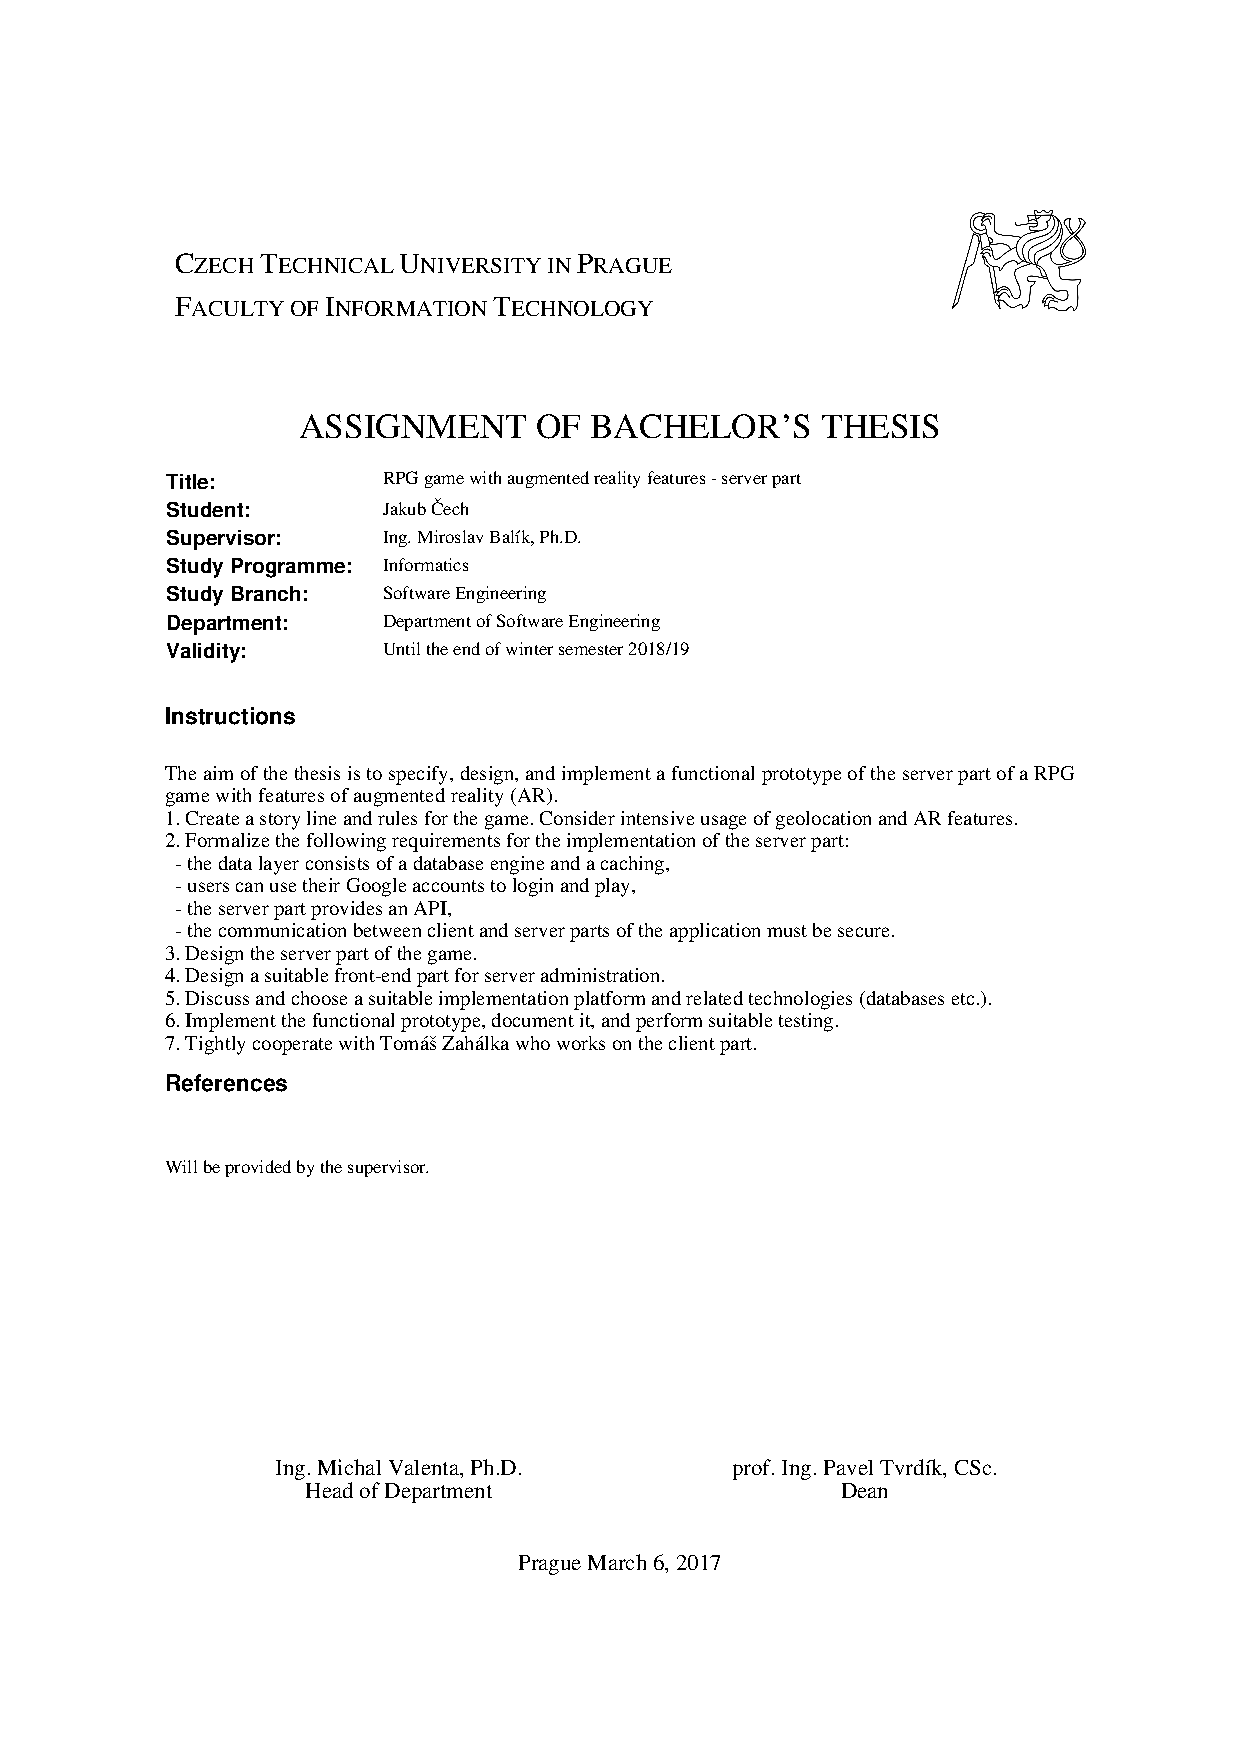
\includepdf[pages={1}]{pdfs/official_assignment.pdf}
	%\newacronym{CVUT}{{\v C}VUT}{{\v C}esk{\' e} vysok{\' e} u{\v c}en{\' i} technick{\' e} v Praze}
	%\newacronym{FIT}{FIT}{Fakulta informa{\v c}n{\' i}ch technologi{\' i}}
	
	\setsecnumdepth{part}
	\chapter{Introduction}
	The world of mobile devices is quickly evolving. Smartphones and tablets are becoming more powerful and not only in terms of computational power and available memory. Nowadays, mobile devices are packed with various sensors. It is possible to acquire data from GPS (Global Positioning System) to quickly determine device’s position. This opens us door to augmented
reality (AR) applications. 

Surprisingly, there are not many existing augmented reality games on the~market. Thanks to couple successful AR games in recent years, which I will explore later,  public awareness of this genre rapidly rose.

In my bachelor thesis, I will create the~server part of a~role-playing augmented reality game. I will work in cooperation with Tomáš Zahálka, who works on the~client part. I will design and implement a~prototype, test it and deploy it on a~virtual private server.

	
	
	\setsecnumdepth{all}	
	\chapter{Project overview}
	\section{Goals of the Thesis}
The thesis is mainly focused on practical game server development. In the research part, I will analyze existing augmented reality games, research available database management systems and explore frameworks used for server development.

In the practical part, I will specify features and requirements of the server. The goal is to support operations the mobile client might need for seamless gaming experience. These operations include for example getting game objects near a player, or login. The main goal is to implement server's functionality to communicate with clients, parse their requests and respond in valid format. The underlying goals include the need to use a database, caching, and communication with external services. Lastly, the game server prototype should be tested and deployed.	

\section{Game Description}
This is a role-playing mobile game with augmented reality features. Player becomes a character in an invisible alternative reality. He can explore the new, magical world using his phone which displays a map with objects around him. Player can discover monsters, like goblins or skeletons, and fight them to death for a reward. As he gains more experience and gold, he can buy himself more powerful weapons and armor in a shop. Tired of running in the outside world? Player can exchange his real money for in-game gold.

For prototyping purposes, some described features are limited. All available actions are specified in \textit{Features} section of Requirements \ref{section:fr}.

\section{Game Story}
Fiddle
	
	\chapter{Analysis}
	
\section{Similar solutions}

	\subsection{Parallel Kingdom - Age of Ascension}
	This game was on market for 8 years (2008-2016). Parallel Kingdom is a closest solution to ours.
	
	
	”Parallel Kingdom is a mobile, location based, massively multiplayer game that uses GPS
	location and Google Maps to place users in a virtual world. Parallel Kingdom is the first
	location based RPG for the iOS and Android platforms. The game is set in a virtual world
	or ”Parallel Kingdom” where users claim their territories based on their GPS location or by making friends who invite them to travel to new places. Parallel Kingdom is a freemium
	game and utilizes a virtual goods revenue model.”
	
	\subsection{Ingress}
	Developed by Niantic, which was then part of Google, this game was released in 2013 for
	Android and in 2014 for iOS.[4] It is a location based, massively multiplayer game. A player have to choose one of the two factions, Enlightened or Resistance, and then as a part of his 	team capture regions of the game map. A faith of each faction relies on players’ cooperation. Thanks to that players meet in real life and coordinate their actions.
	
	Ingress was the first very successful augmented reality game with more than 10 000 000
	installs.
	
	\subsection{Pokémon GO}
	After its success with Ingress, Niantic started working on a new game Pokemon GO. Once
	released, the game became incredible hit. Even though the game faced many problems during
	its launch, mainly caused by the unexpected success and more active users than Pokémon
	GO was able to handle, in the first 80 days Pokémon GO reached about 550 millions downloads and earned about \$470 million.
		
	The game is very similar to Ingress and uses the same crowd-sourced geographical data.
	
\section{Use Cases}
	\subsection{Actors}
		\begin{figure}[h]	
			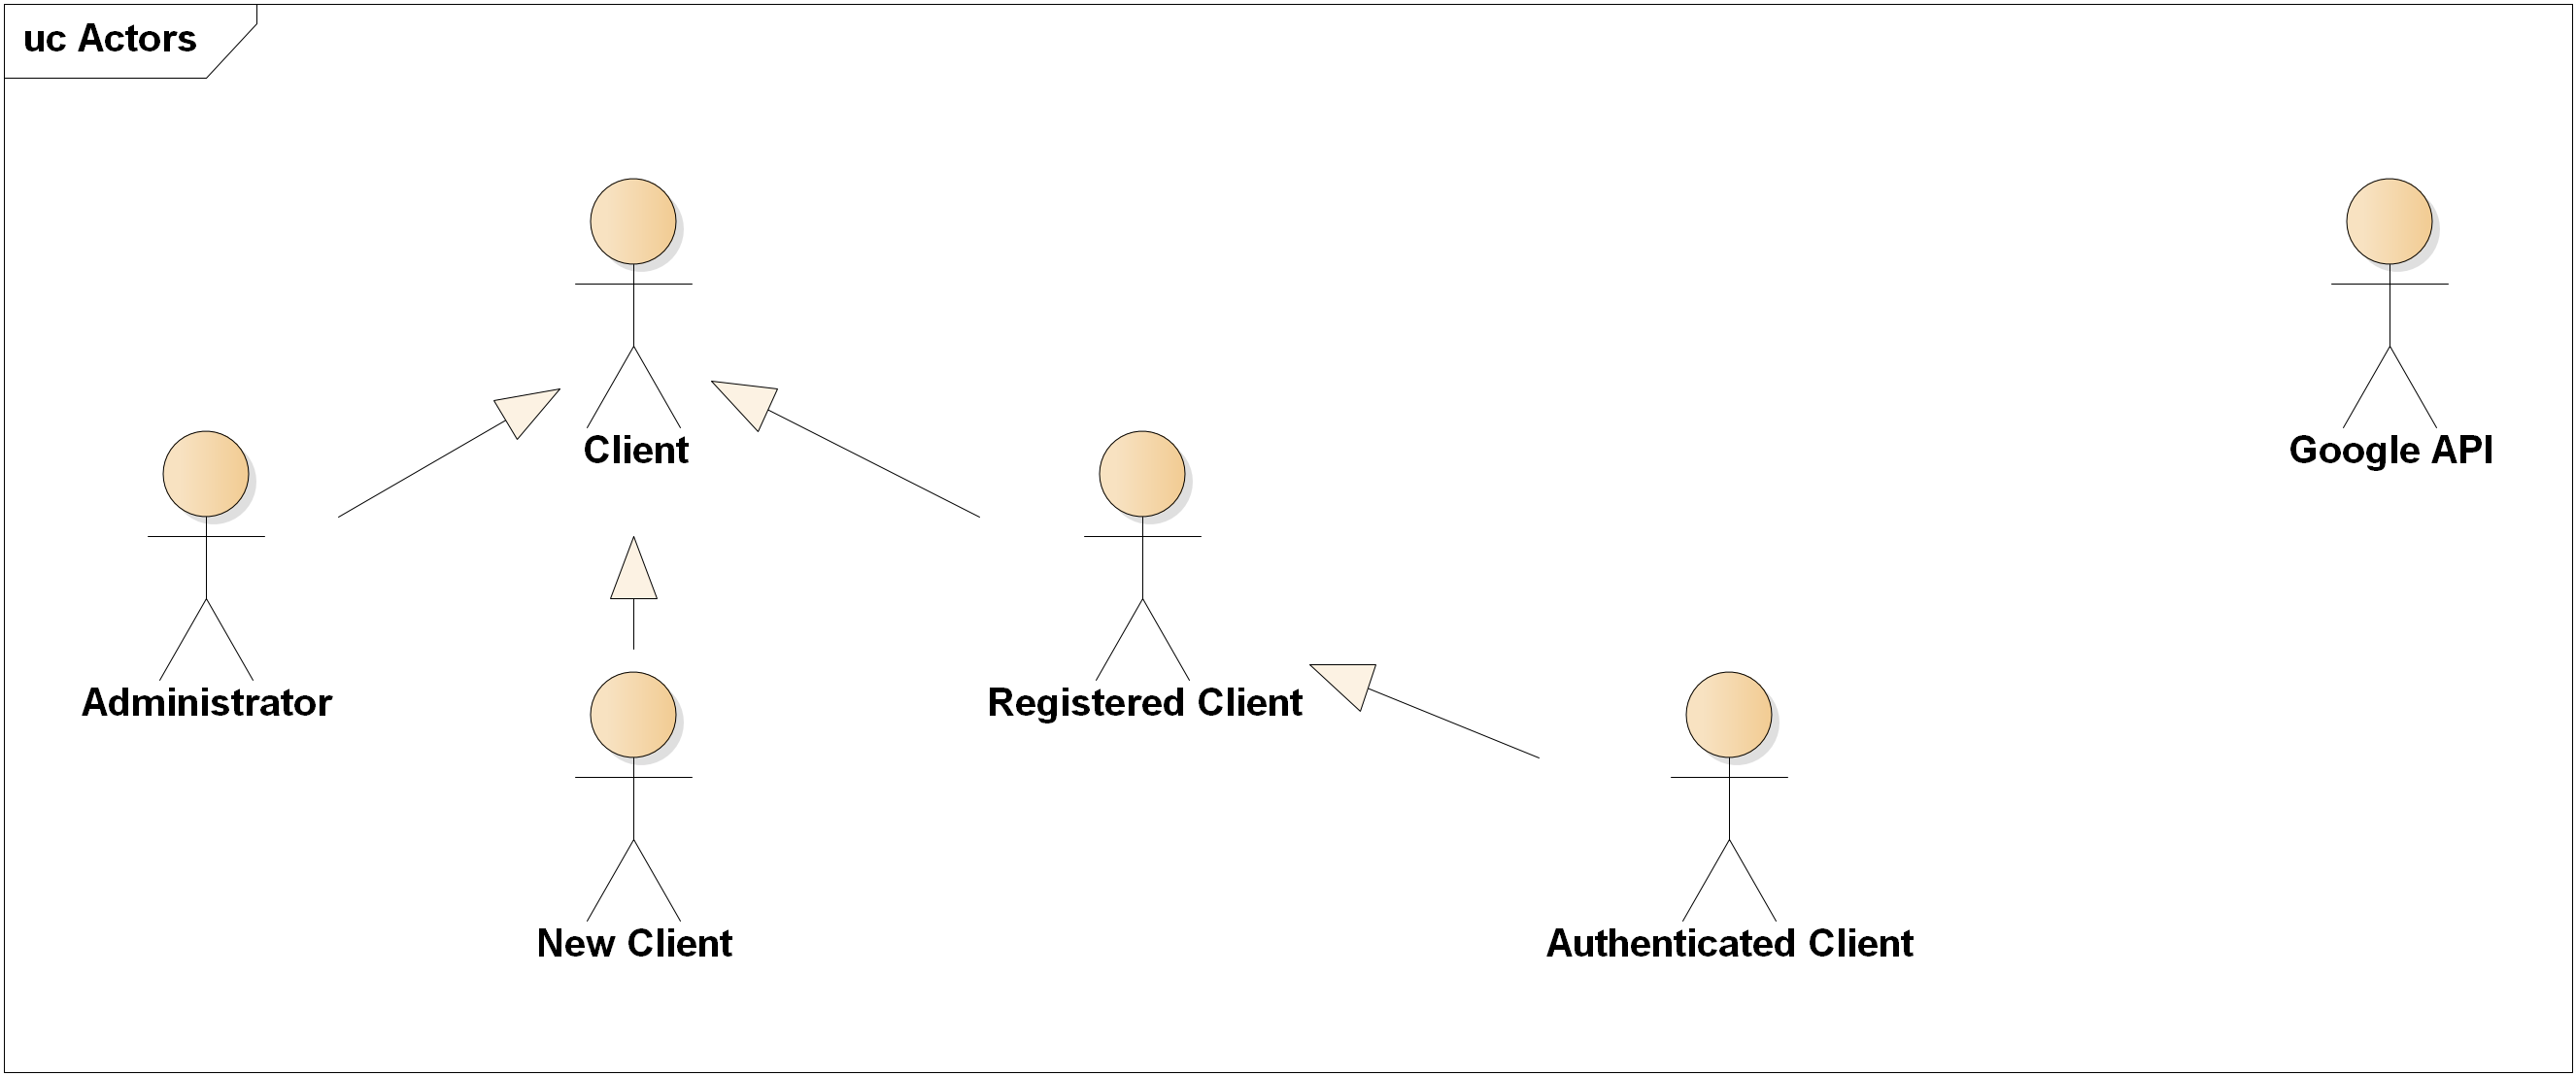
\includegraphics[width=\textwidth]{figures/UC_Actors}
			\centering			
			\caption{Use Case
				 Diagram -- Actors}
			\label{fig:ucactors}
		\end{figure}
		\noindent Actor is a role played by a user or other system that interacts with the server. The most general role is \textit{Client} and anyone who accesses the server through API is considered to play either this role or any of its children. From now on, the terms client and user will be used interchangeably. Refer to Figure \ref{fig:ucactors} for the role hierarchy.
		
		\textit{Administrator} is a client who has privilege to create and maintain the functionality of the game. \textit{New Client} is a user who is not yet registered and probably accesses the game for the first time. \textit{Registered Client} is the default role for a user who already has a valid account but is not logged in. Lastly, \textit{Authenticated Client} has all the required privileges to play the game. This client will be refereed to as \textit{player}. The last main actor is Google API which provides the access to Google services. 		

	\subsection{Authentication}	
	\begin{figure}[h]	
		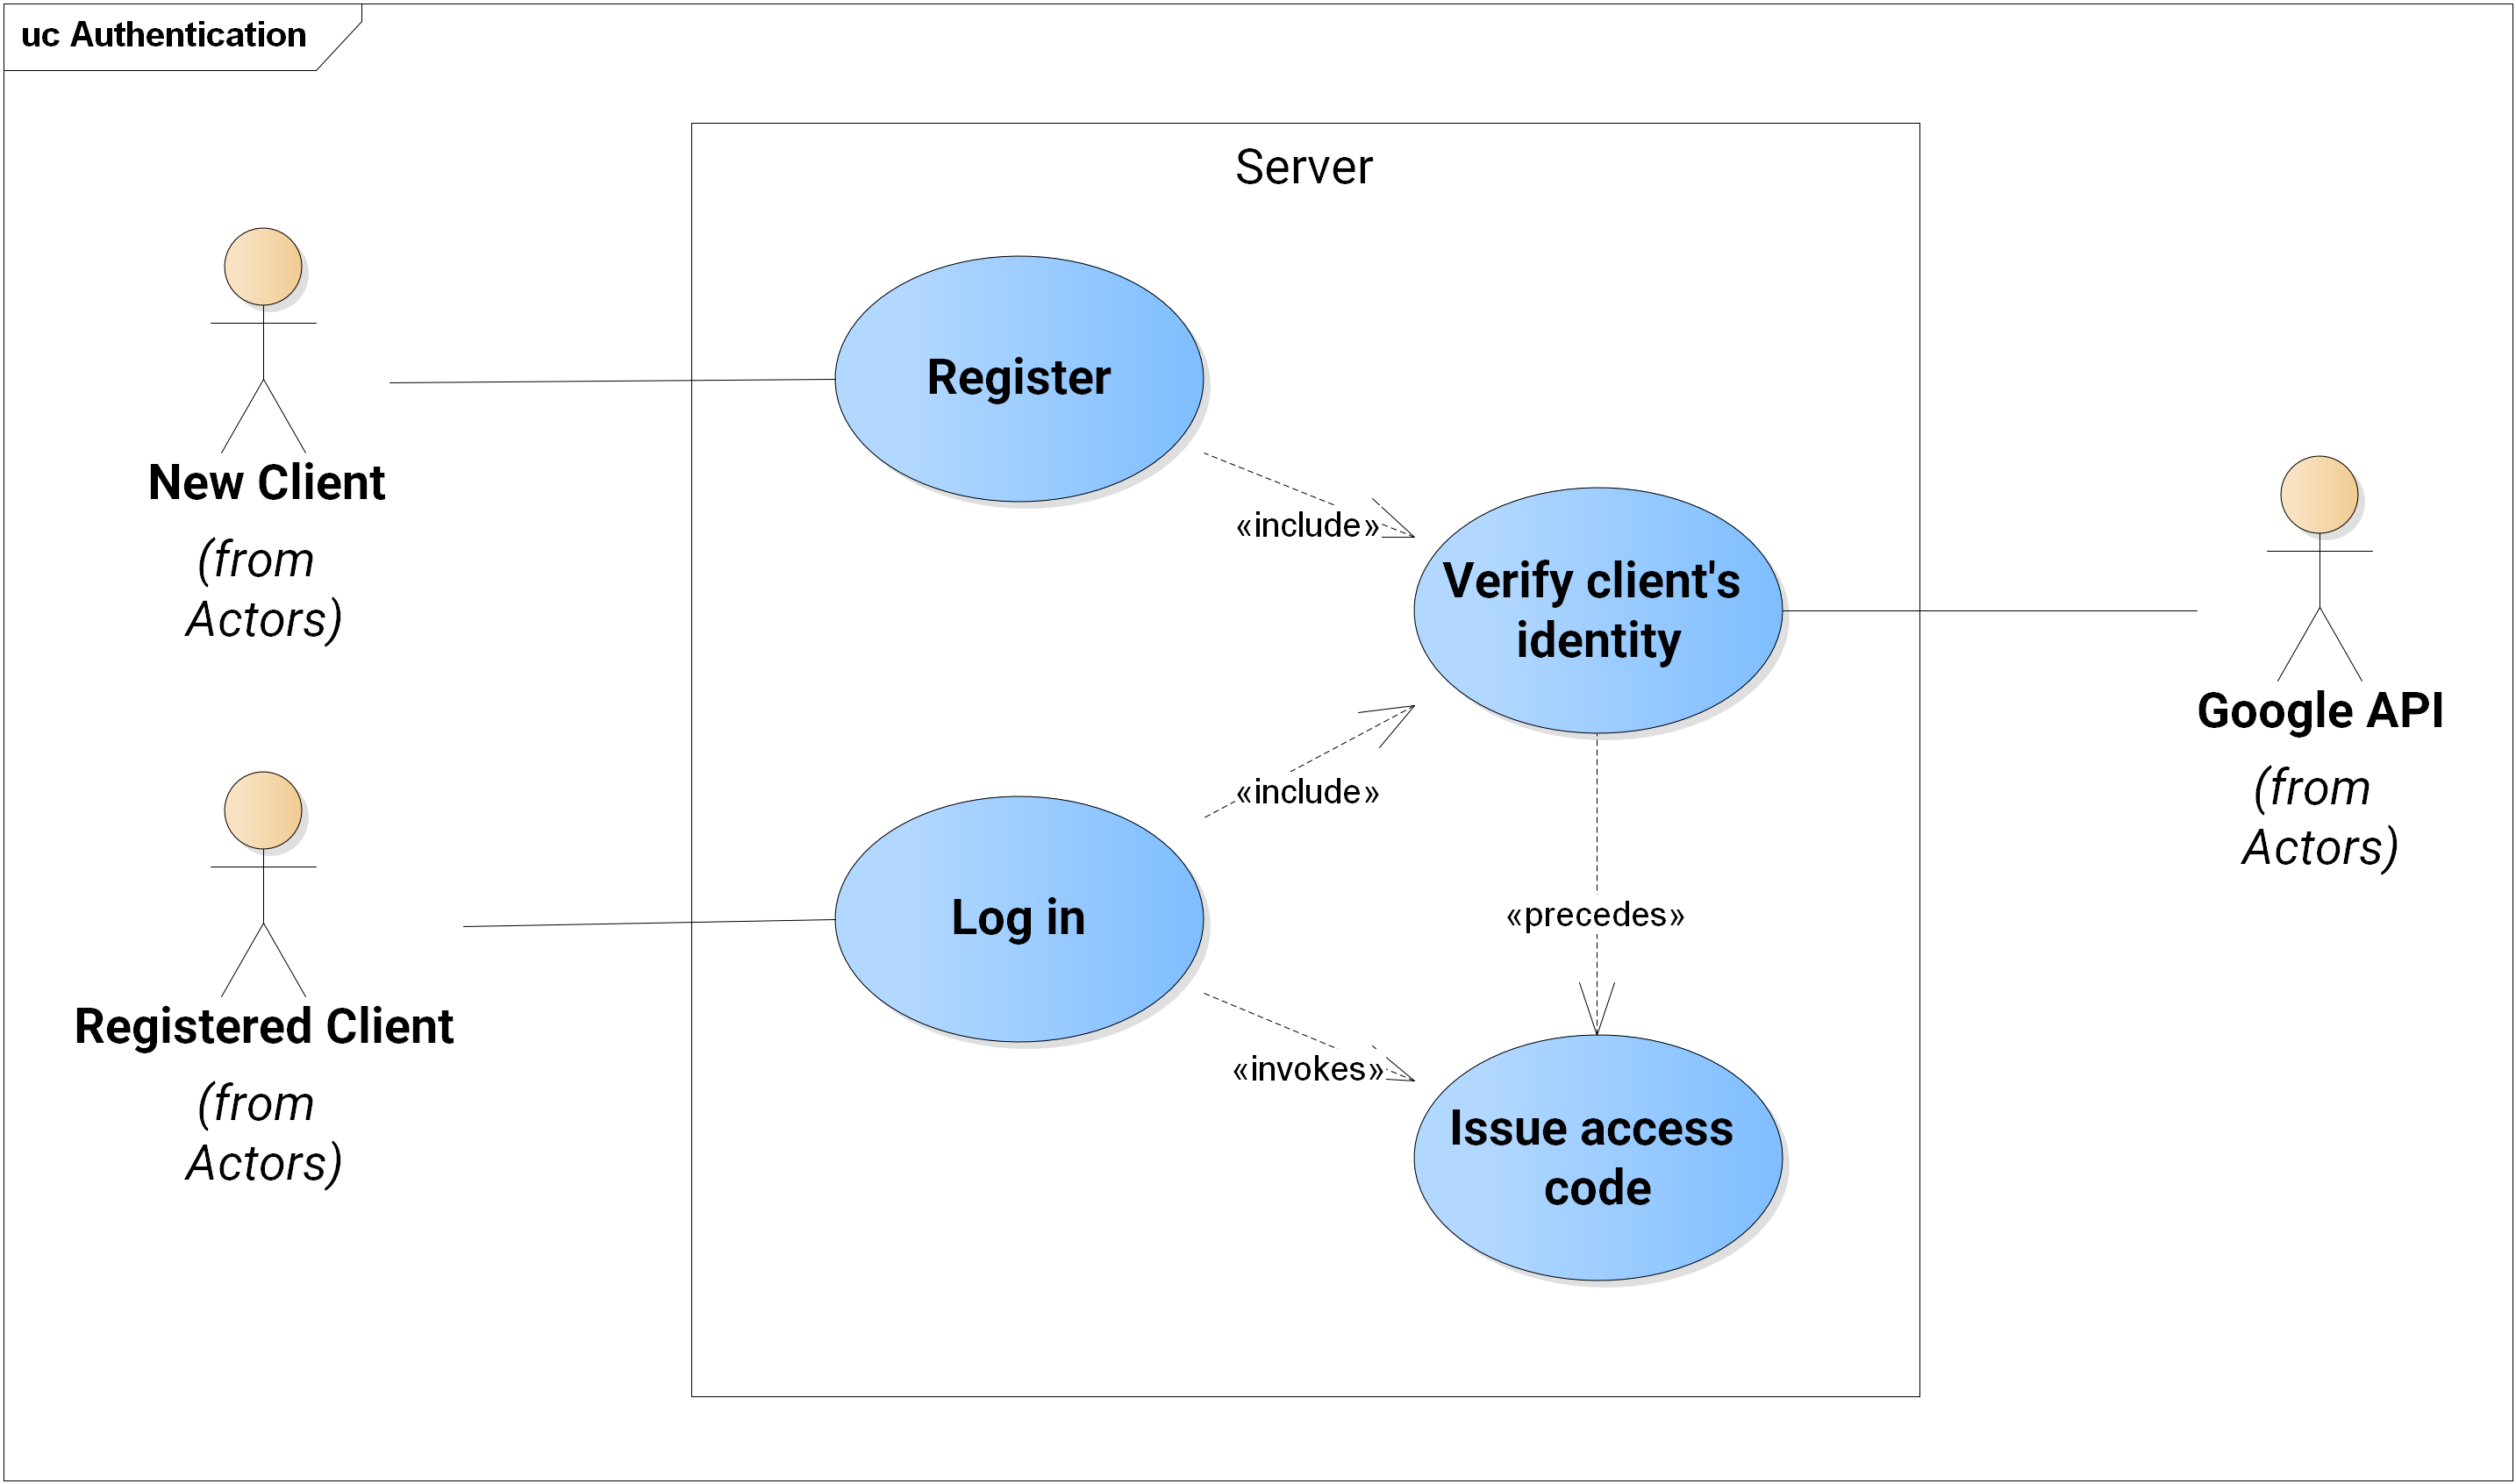
\includegraphics[width=\textwidth]{figures/UC_Authentication}
		\centering			
		\caption{Use Case Diagram -- Client's authentication}
		\label{fig:ucauth}
	\end{figure}
	\noindent Authentication use cases user performs to get promoted to more privileged roles. The basic transition flow is \textit{New Client} $\rightarrow$ \textit{Registered Client} $\rightarrow$ \textit{Authenticated Client}. See Figure \ref{fig:ucauth}.
	
	\begin{itemize}
		\item \textbf{Register} \\
		The only choice \textit{New Client} has is to register a new account. He uses provides his Google identity and chooses an username. After his identity is verified, the server creates a new profile and logs the user in.
		
		\item \textbf{Log in} \\
		The \textit{Registered Client} must log in before he can access any of the game features. He provides his Google identity which is then verified and matched to an account. An access code is issued for the future identification within the session.		
		
		\item \textbf{Verify user's identity} \\
		Proper verification is needed when the game server receives a Google identity of a user. The server contacts the \textit{Google API} which responds with user's personal information if the identity is valid.
		
		\item \textbf{Issue access code} \\ 
		This use case is invoked during login process. Server issues a unique access code to the user. Only \textit{Authenticated Client} has such code.
	\end{itemize}
	
	\subsection{Actions}	
		\begin{figure}[h]	
			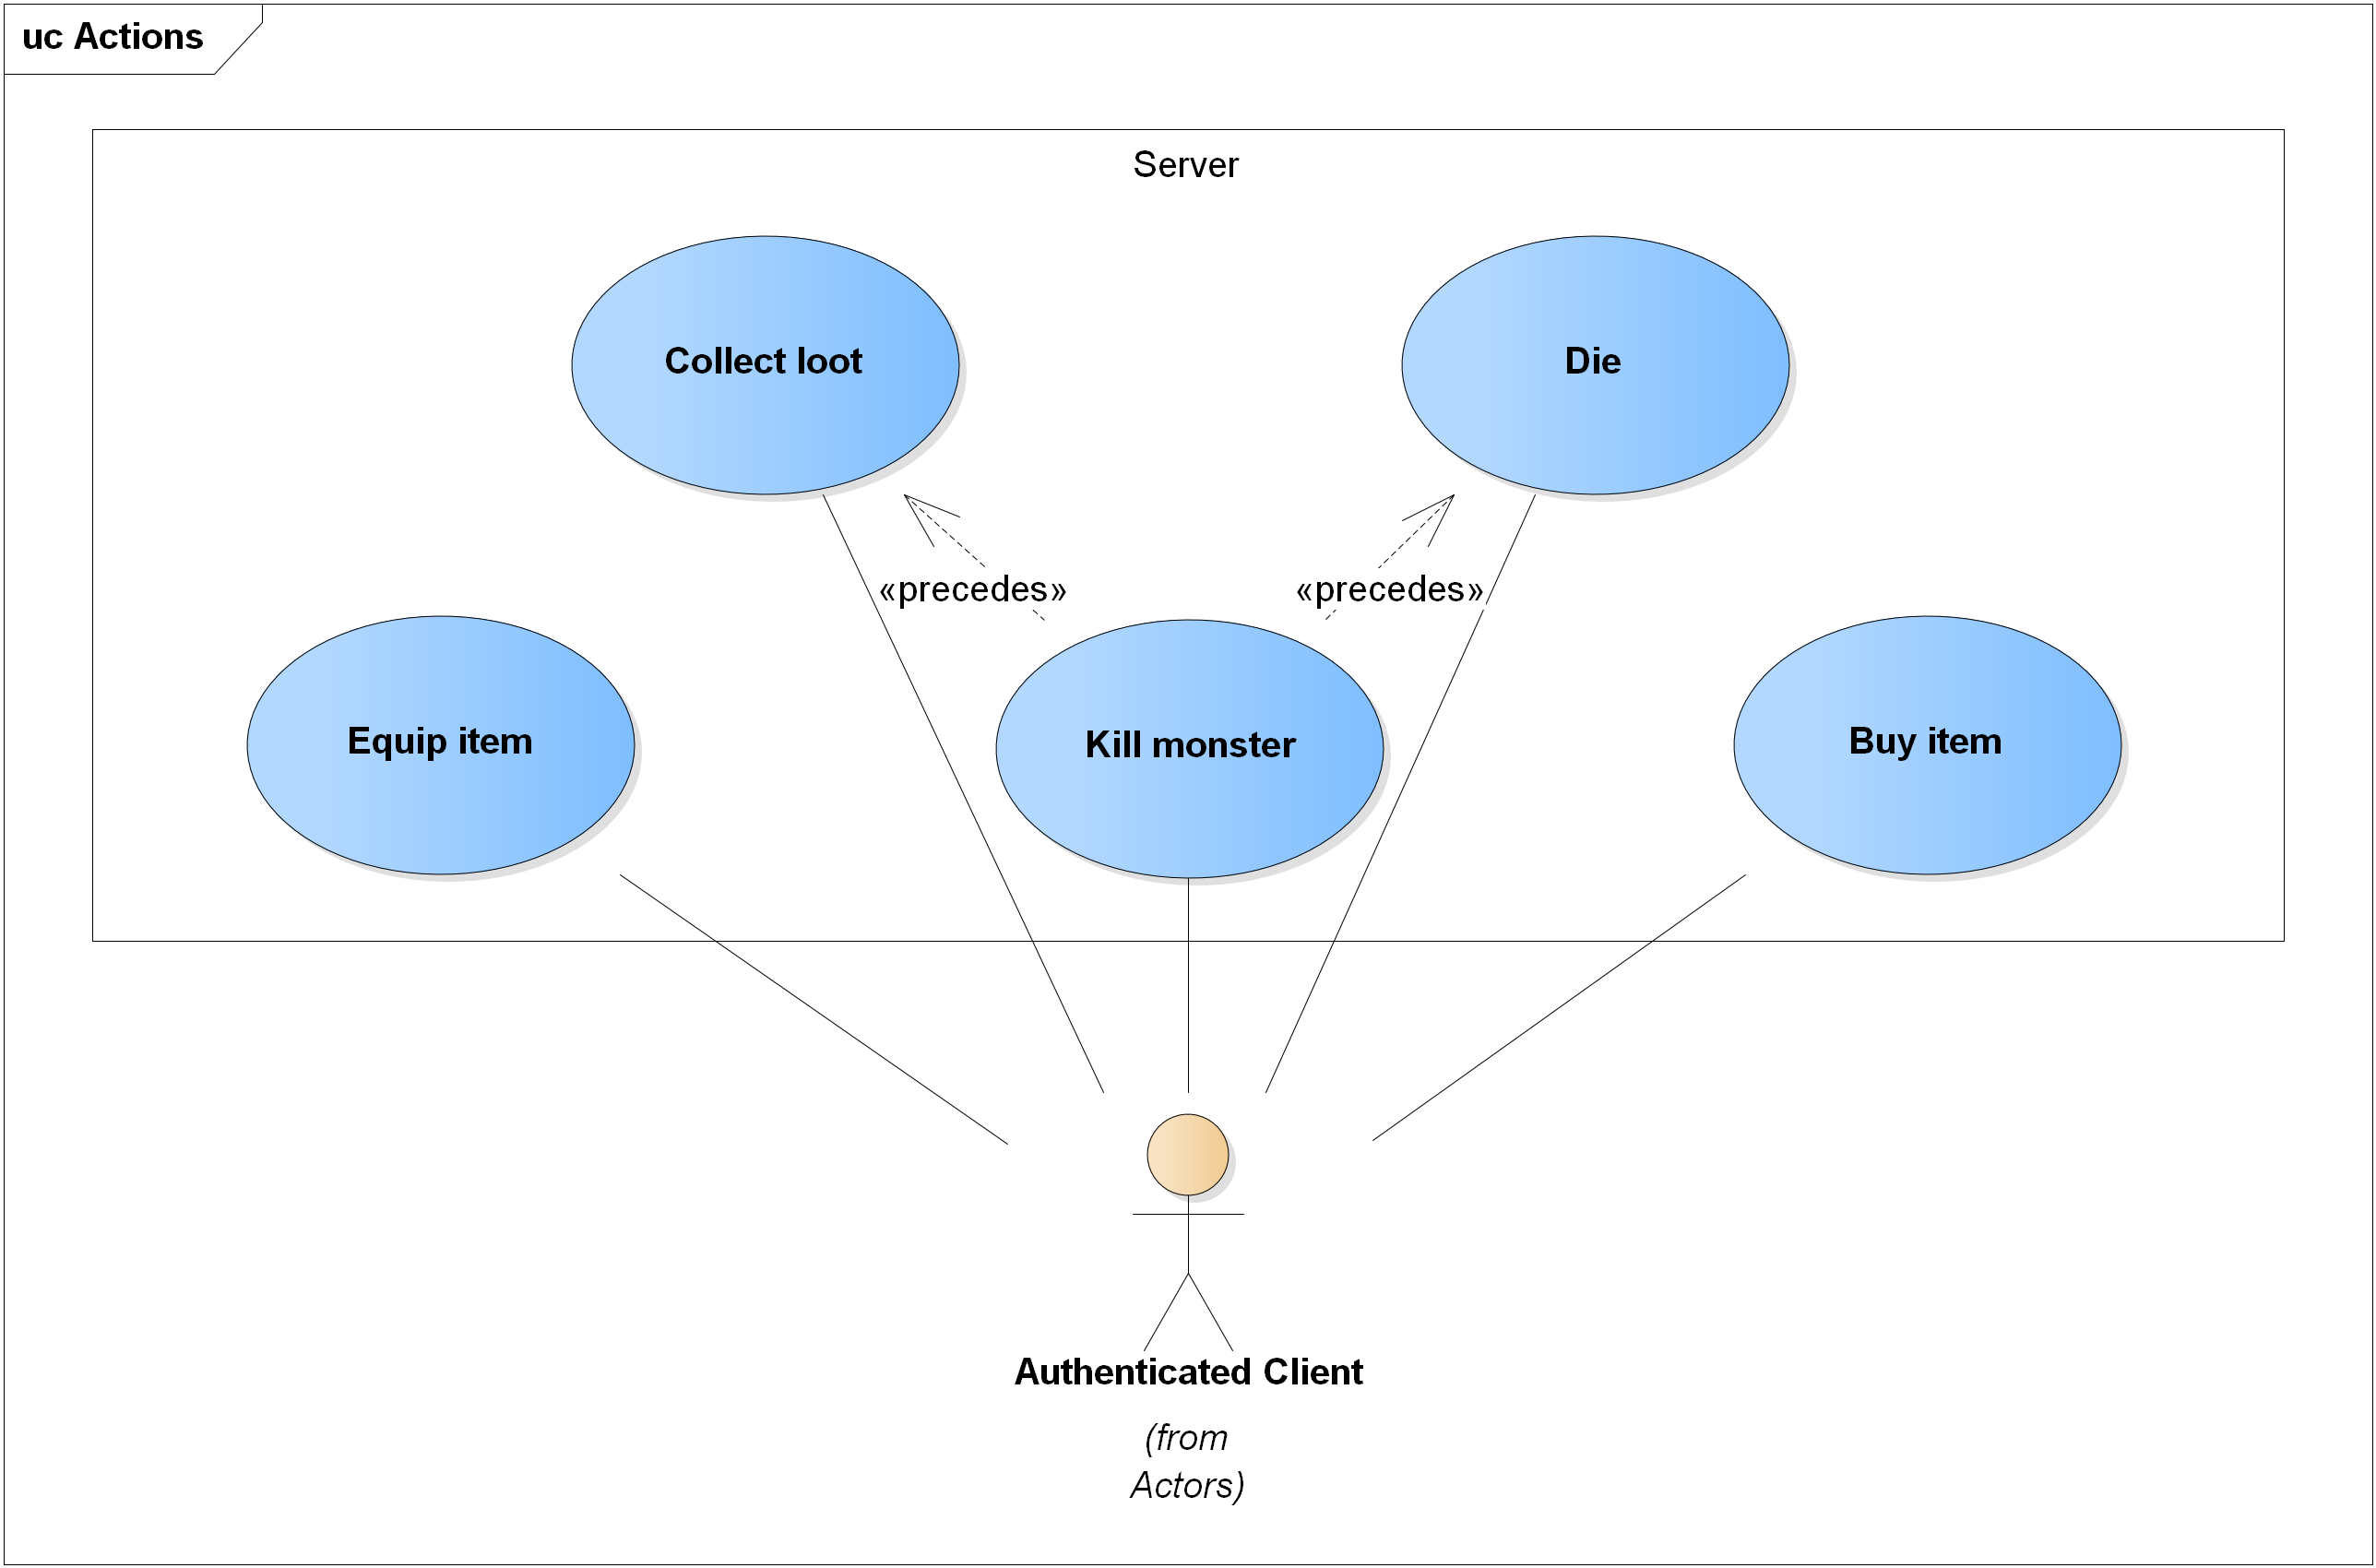
\includegraphics[width=\textwidth]{figures/UC_Actions}
			\centering			
			\caption{Use Case Diagram -- Player's actions}
			\label{fig:ucactions}
		\end{figure}
		\noindent Action is an event triggered by player's interaction with a game object. See the diagram in Figure \ref{fig:ucactions}.
		
		\begin{itemize}
			\item \textbf{Equip item} \\
			A player wants to equip an item from his inventory. The item will be assigned to a specific slot. For example the player equips a sword to his right hand.
			
			\item \textbf{Buy item} \\
			A player wants to exchange gold in a shop for an item he chooses. When the purchase is finished, the player receives the item to his inventory.
			
			\item \textbf{Kill monster} \\
			A player wants to kill monsters to progress in the game. If he successfully kills the monster, he is rewarded with gold and experience
			
			\item \textbf{Collect loot} \\
			This action must be preceded by the \textit{Kill monster} use case. A player can choose to collect loot from the monster he killed.
			
			\item \textbf{Die} \\
			This action must be preceded by the \textit{Kill monster} use case. A player who lost his fight against a monster dies and is punished with some penalty.		
		\end{itemize}
	
	\subsection{Miscellaneous}
	\begin{figure}[h]	
		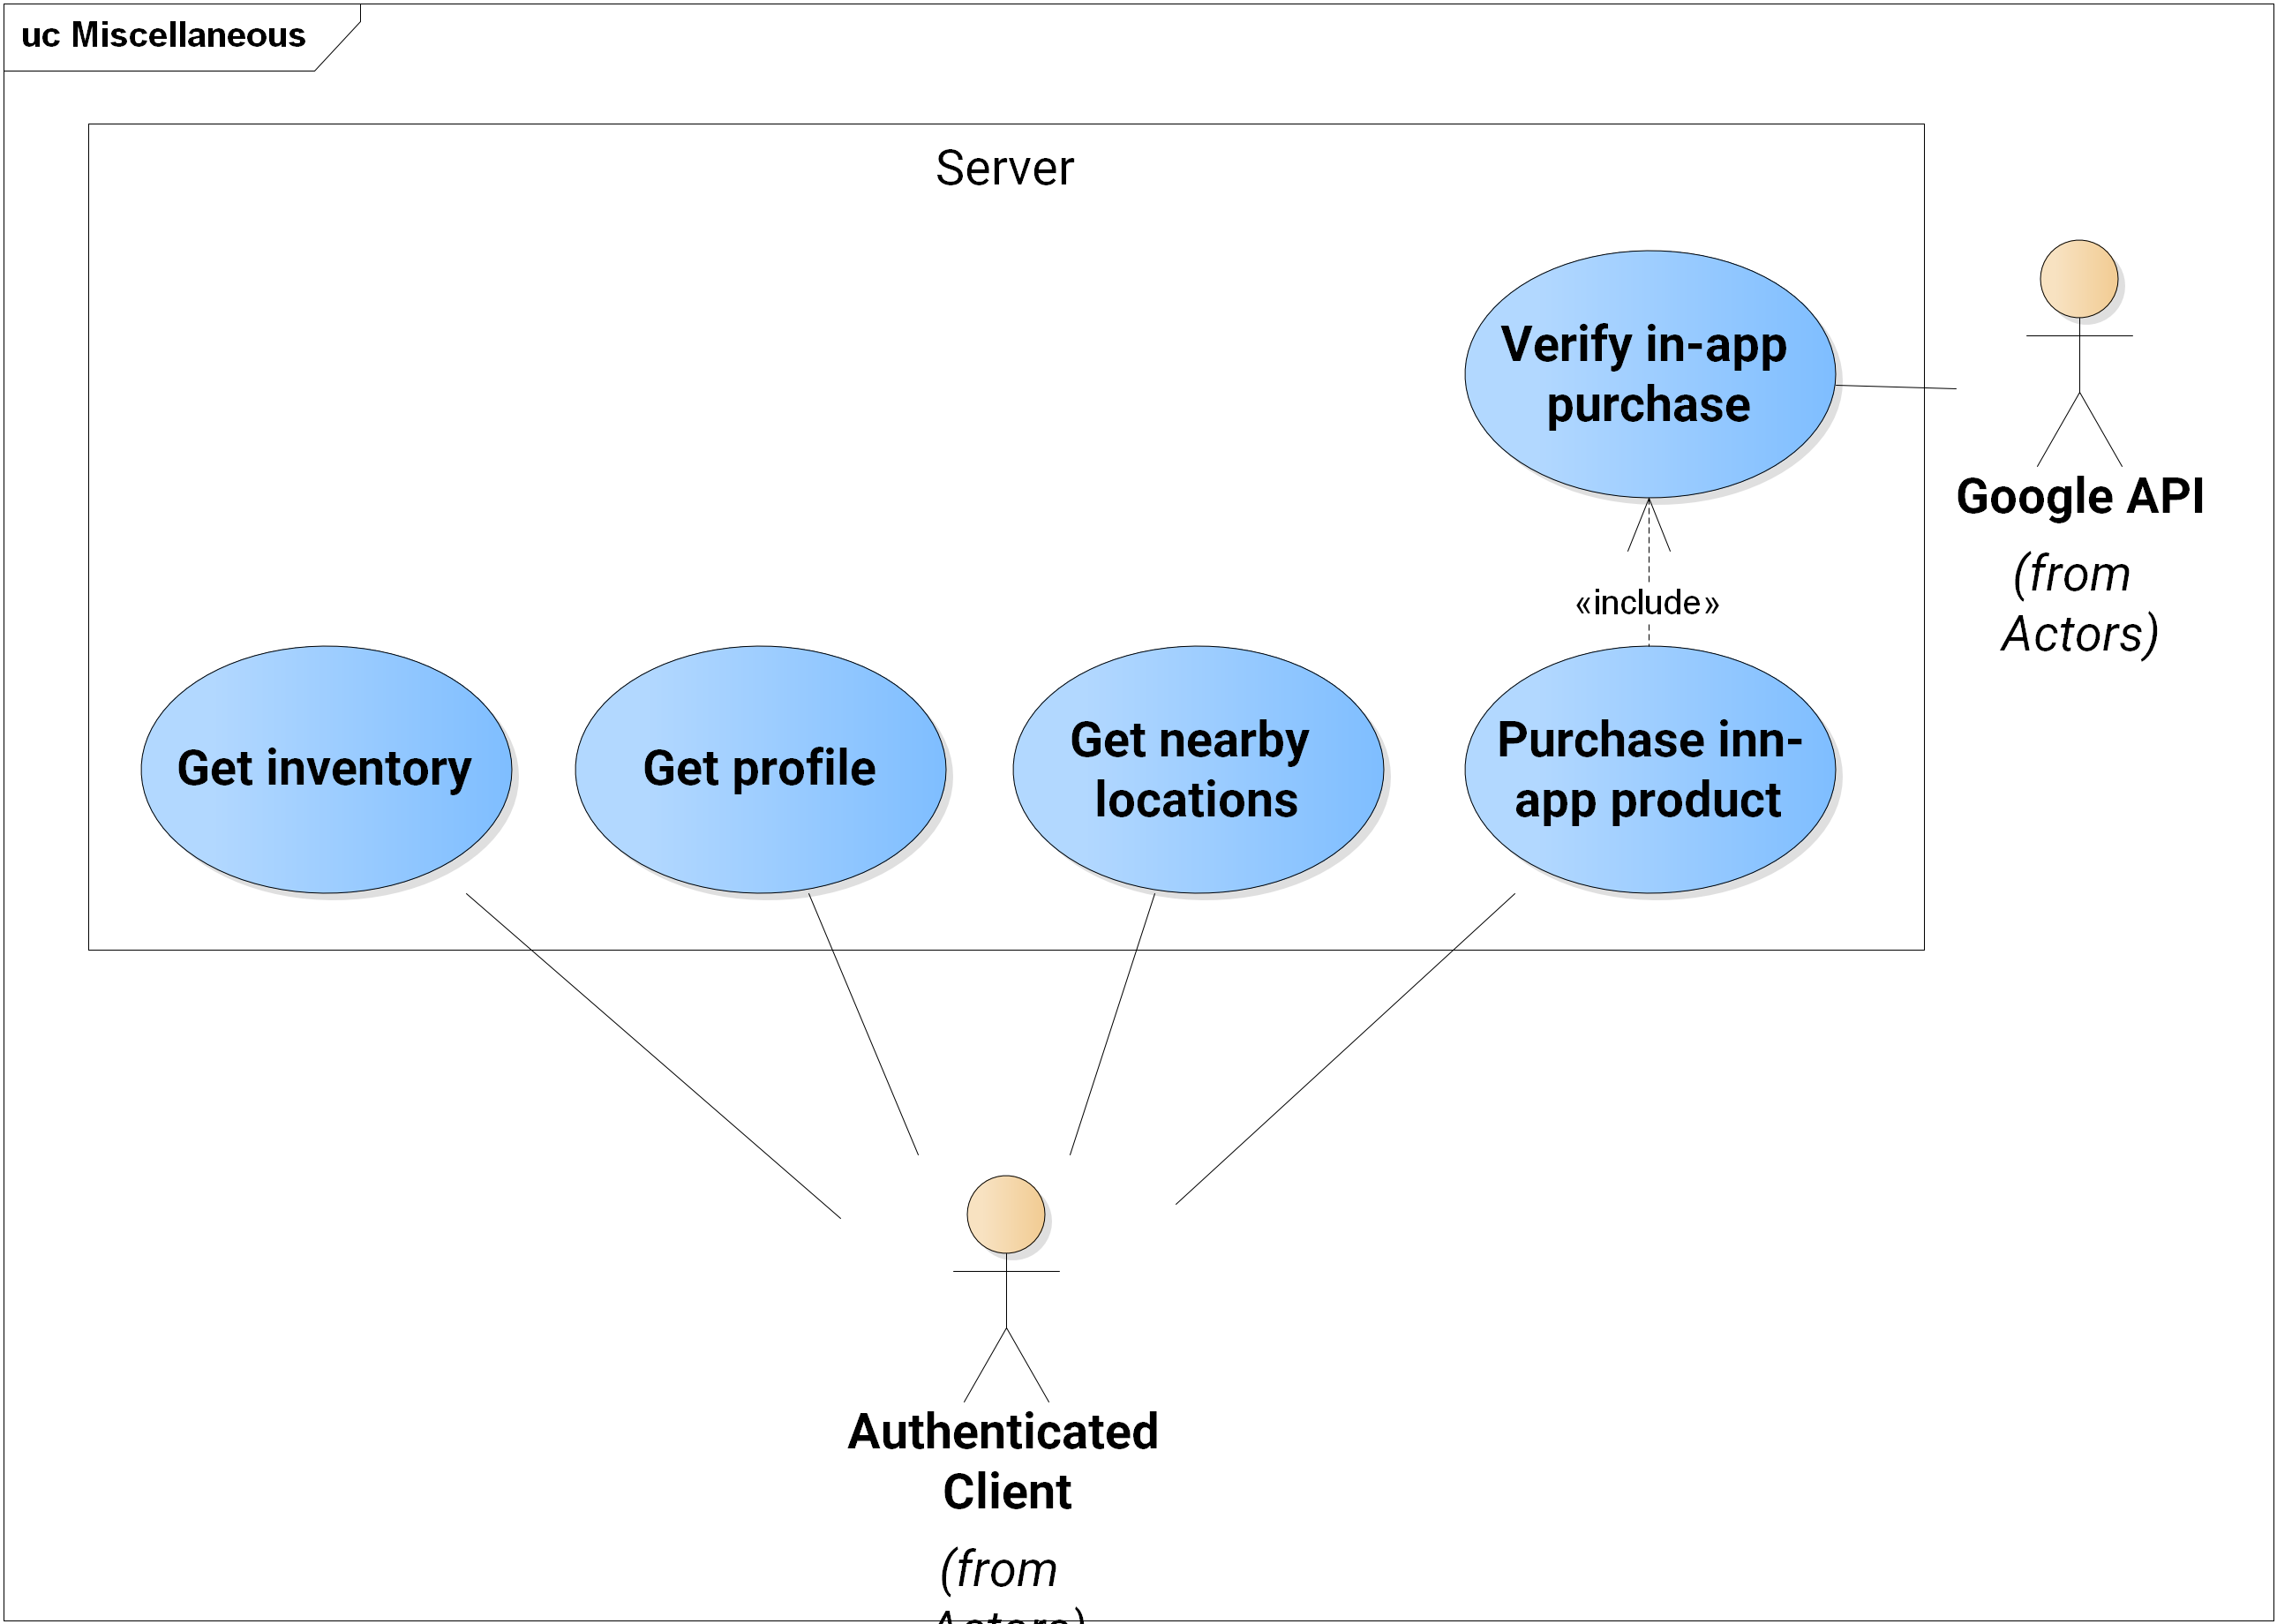
\includegraphics[width=\textwidth]{figures/UC_Miscellaneous}
		\centering			
		\caption{Use Cases: Miscellaneous}
		\label{fig:ucmisc}
	\end{figure}
	The following use cases mainly cover requests made by client application. See the diagram in Figure \ref{fig:ucmisc}.
	\begin{itemize}
		\item \textbf{Get inventory}\\
		The application requests all items the player owns. It is also possible to retrieve all the player's equipment with each item assigned to some slot.
		
		\item \textbf{Get profile}\\
		A client may need to synchronize its internal state of the players profile with the server. The application is provided with complete state of the player's profile including attributes like health, gold, and experience.
		
		
		\item \textbf{Get nearby locations}\\
		This is a critical functionality of the server. A client asks for game locations near his coordinates. The server provides such locations along with their associated game objects.
		
		
		\item \textbf{Purchase in-app product}\\
		The application supports micro-transactions. Since the purchase is made client-side, the application has to notify the server about the purchase and give the bought product to the player. 
		
		
		\item \textbf{Verify in-app purchase}\\
		During the previous use case (\textit{Purchase in-app product}), the server verifies if the purchase is valid and not fake, canceled, or already accounted. The verification process contacts \textit{Google API} which confirms the validity.
		
		
	\end{itemize}
	

	\subsection{Administration}
	\begin{figure}[h]	
		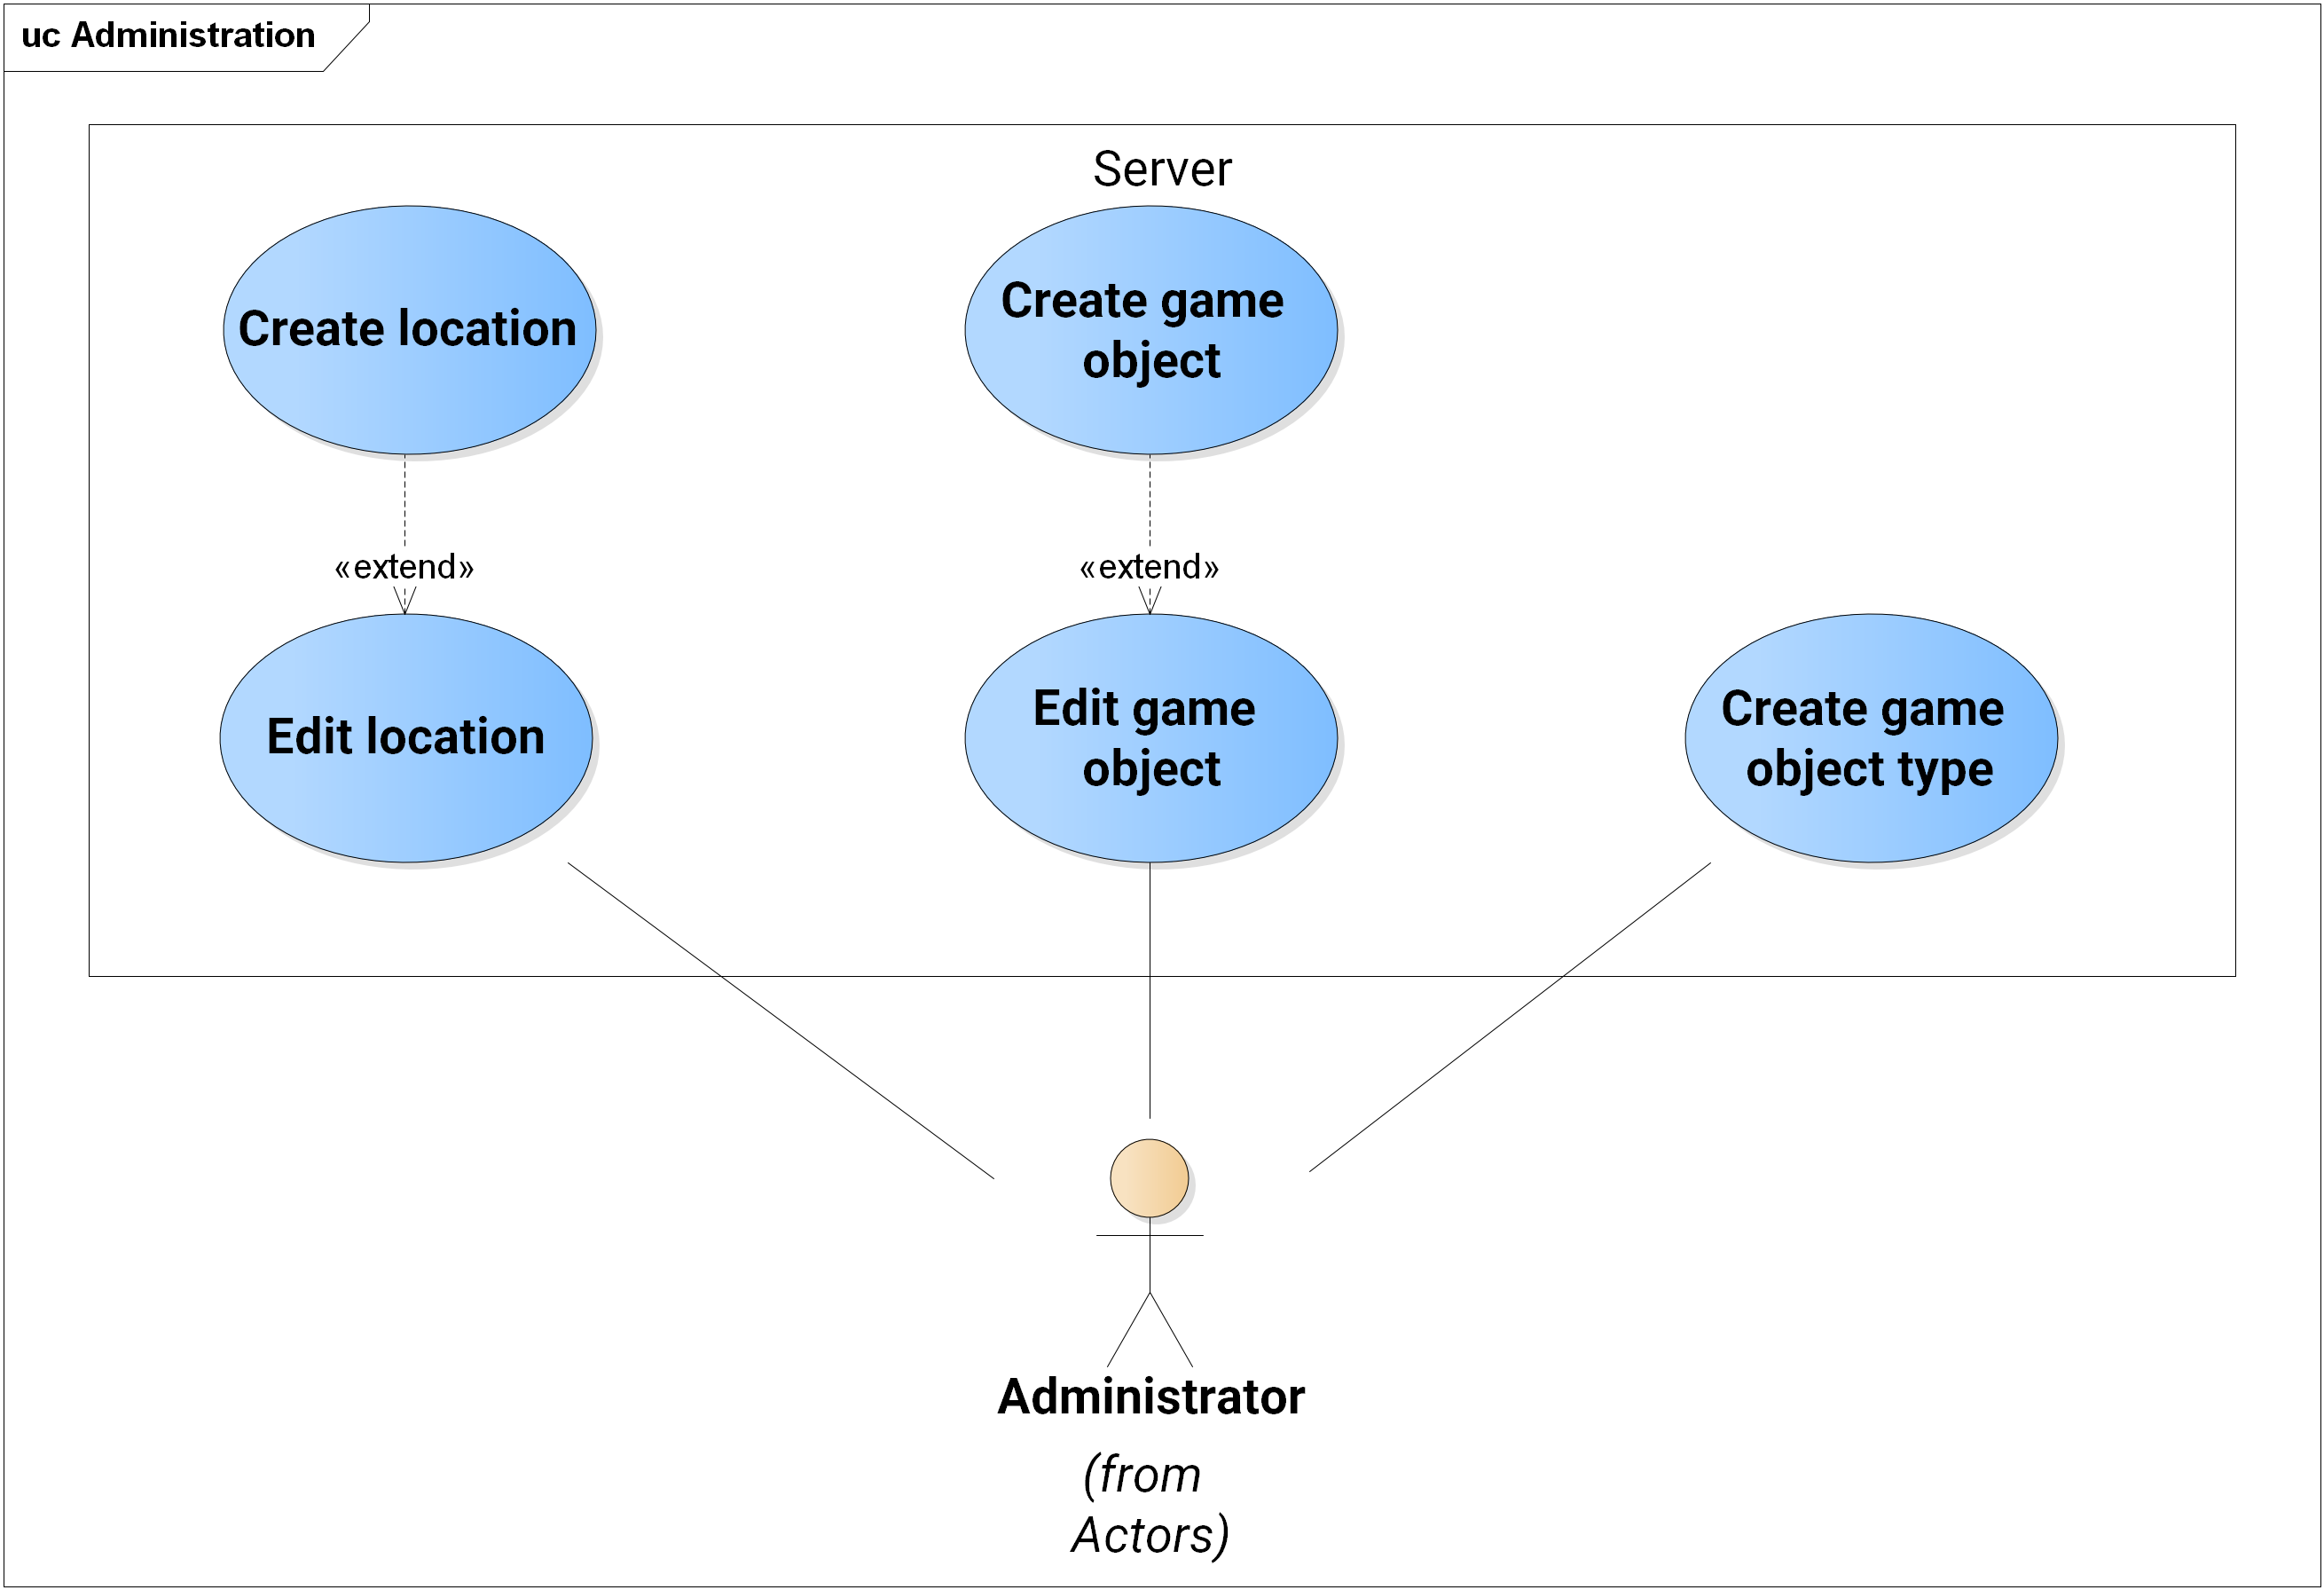
\includegraphics[width=\textwidth]{figures/UC_Administration}
		\centering			
		\caption{Use Cases: Administration}
		\label{fig:ucadmin}				
	\end{figure}	
	\noindent Since the game is not static during its lifetime, people in charge of the changes needs an easy way to add new locations and maintain game objects. These use cases are described in Figure \ref{fig:ucadmin}.
	
	
\section{Requirements}

	\subsection{Functional Requirements}
		\subsubsection*{Rules}
		\begin{enumerate}
			\item \textbf{The server must provide API to clients} \\
			The key requirement for the server is to allow receiving HTTP(S) requests. When processed, the server responds in JSON format.
						
			\item \textbf{The player's character has attributes} \\
			The character has a set of attributes, including health, experience, level, and owned gold. Maximum health increases with level. The experience is rewarded after certain actions, e.g. after killing a monster. The gold is primary in-game currency.
			  
			\item \textbf{A player can own items} \\
			A player has an inventory which can contain various types of items. The item can be for example sword, potion, armor etc.
			
			\item \textbf{A game object has a type and inherits all its properties} \\
			The type of game object specifies allowed actions, its attributes, default name and description.			
			
			\item \textbf{A game object can be a monster} \\
			The monster can be killed but can also inflict damage to the player. It has its own inventory and there's a reward for killing the monster in a form of gold and experience.
			
			\item \textbf{A game object can be a shop} \\
			The shop can contain several items with specified price.  
			
			\item \textbf{A game object can be an item} \\	
			The item can be one of the many objects useful to a player. Examples of the items are health potion, sword, armor, necklace and similar.
			
			\item \textbf{Each game object has its own inventory} \\
			The inventory contains other game objects. Example of this requirement is a monster with a potion and a sword in its inventory; both will be given to the player who kills the monster.  
			
			\item \textbf{The server stores a list of predefined locations} \\	
			Real geographic locations for the game objects are stored on the server to ensure every player has the same location-object pair. 
								
			\item \textbf{A game object can independently exist at many locations} \\
			This requirement aims to help maintain the game objects efficiently by administrators. It allows creating small set of abstract game objects with predefined inventories and other attributes. 
			
			\item \textbf{If a player kills a monster at a location, the monster will be hidden for a period} \\
			To prevent the player from killing the same monster continuously without a need of moving somewhere else, the location should be hidden for a certain period after the kill.
			
			\item \textbf{The server should provide API for administration} \\	
			Such API will be used to manage locations, create and edit game objects or to assign a game object to some locations. It is necessary to protect the administration endpoints from unauthorized access.
					
			\item \textbf{The server must persist player’s profile between sessions} \\
			All the player's attributes, his inventory and equipment must be stored between sessions. Player will continue from the state in which he ended.
			
		\end{enumerate}
		\subsubsection*{Features}
		\begin{enumerate}
			\item \textbf{A player registers and logs in the game using Google account} \\
			For the player's convenience, a Google account is required to play. The server does not have to store or handle any password. Most of the authentication process is delegated to Google servers.
			
			\item \textbf{A client can get nearby game objects based on his location} \\
			The major feature of this application is being location-aware. Server must provide a method to retrieve game locations near the requested latitude and longitude. The "near area" should be circular, defined by its radius; the size have to be carefully chosen so it's big enough to cover client's maps but also small to limit the response size and the spatial search overhead.
			
			\item \textbf{A player can kill a monster} \\
			When the player wins the fight, he will be rewarded by experience and gold. 			
			
			\item \textbf{A player can be killed be a monster} \\
			The player can lose health during the fight with a monster. If the health reaches zero, the player dies and loses an amount of gold based on his level.
			
			\item \textbf{A player can collect items from the monster he killed} \\
			When the player wins the fight, he's offered to collect items from the monster's inventory. He can chose any subset of these items.
			
			\item \textbf{A player can equip an item} \\	
			Many items in the game can be equipped. These items have predefined equipment slot, for example a sword have to be held in hand, an armor worn on chest, shoes put on feet and so on.
						
			\item \textbf{A player can buy object from a shop} \\
			Gold can be exchanged for various items in shops.
			
			\item \textbf{A player can use an item from his inventory} \\
			Some items in the game are consumables. When used, an action defined by the item is executed. For example a health potion heals the player.
			
			\item \textbf{A player can purchase in-app product} \\
			The application allow a user to exchange real-life currency for the in-game one. The server should verify such purchase and add the currency to his profile.
			
		\end{enumerate}
		
		
	\subsection{Non-functional}
	
		\begin{enumerate}
			\item \textbf{The data layer consists of a database engine and a caching} \\
			Game Server never accesses database directly. Data are retrieved from the database upon request and then cached. Upper layers communicate exclusively with cache.		
			
			\item \textbf{The server provides an API for client} \\
			The API support at least following:
			\begin{enumerate}
				\item Retrieve nearby game locations
				\item Create player
				\item Update player's data (inventory, experience, resources, quests progress etc.)
				\item Provide information about a quest 			
			\end{enumerate}
			
			\item \textbf{The communication between client and server parts of the application must be secure} \\
			All data sent from and to a client has to be encrypted.
	
			\item \textbf{Client can only connect to a Connection Server} \\
			Several Connection Servers exist to prevent a bottle-neck. Client selects the Connection Server by an algorithm. Client does not have an access to any other part of the server.
		\end{enumerate}
	\subsection{System and Interface}
	
		\begin{enumerate}
			\item \textbf{System uses Java 8 SE as an execution environment} \\
			
			\item \textbf{Operating system for the server is Debian 8} \\
			
			\item \textbf{Database engine is MySQL} \\
			
			\item \textbf{Cache engine is Redis} \\
		\end{enumerate}
	
\section{Technology}

	\subsection{Frameworks}
	
	
	\chapter{Design}
	\section{Components}
The~game server is divided into separate components. Many instances of a~component can run at~the~same time. Component, and even instances, can be distributed among many machines; this feature renders the~whole server easily scalable. Refer to Figure \ref{fig:components} for a~component diagram.

\begin{figure}[h]	
	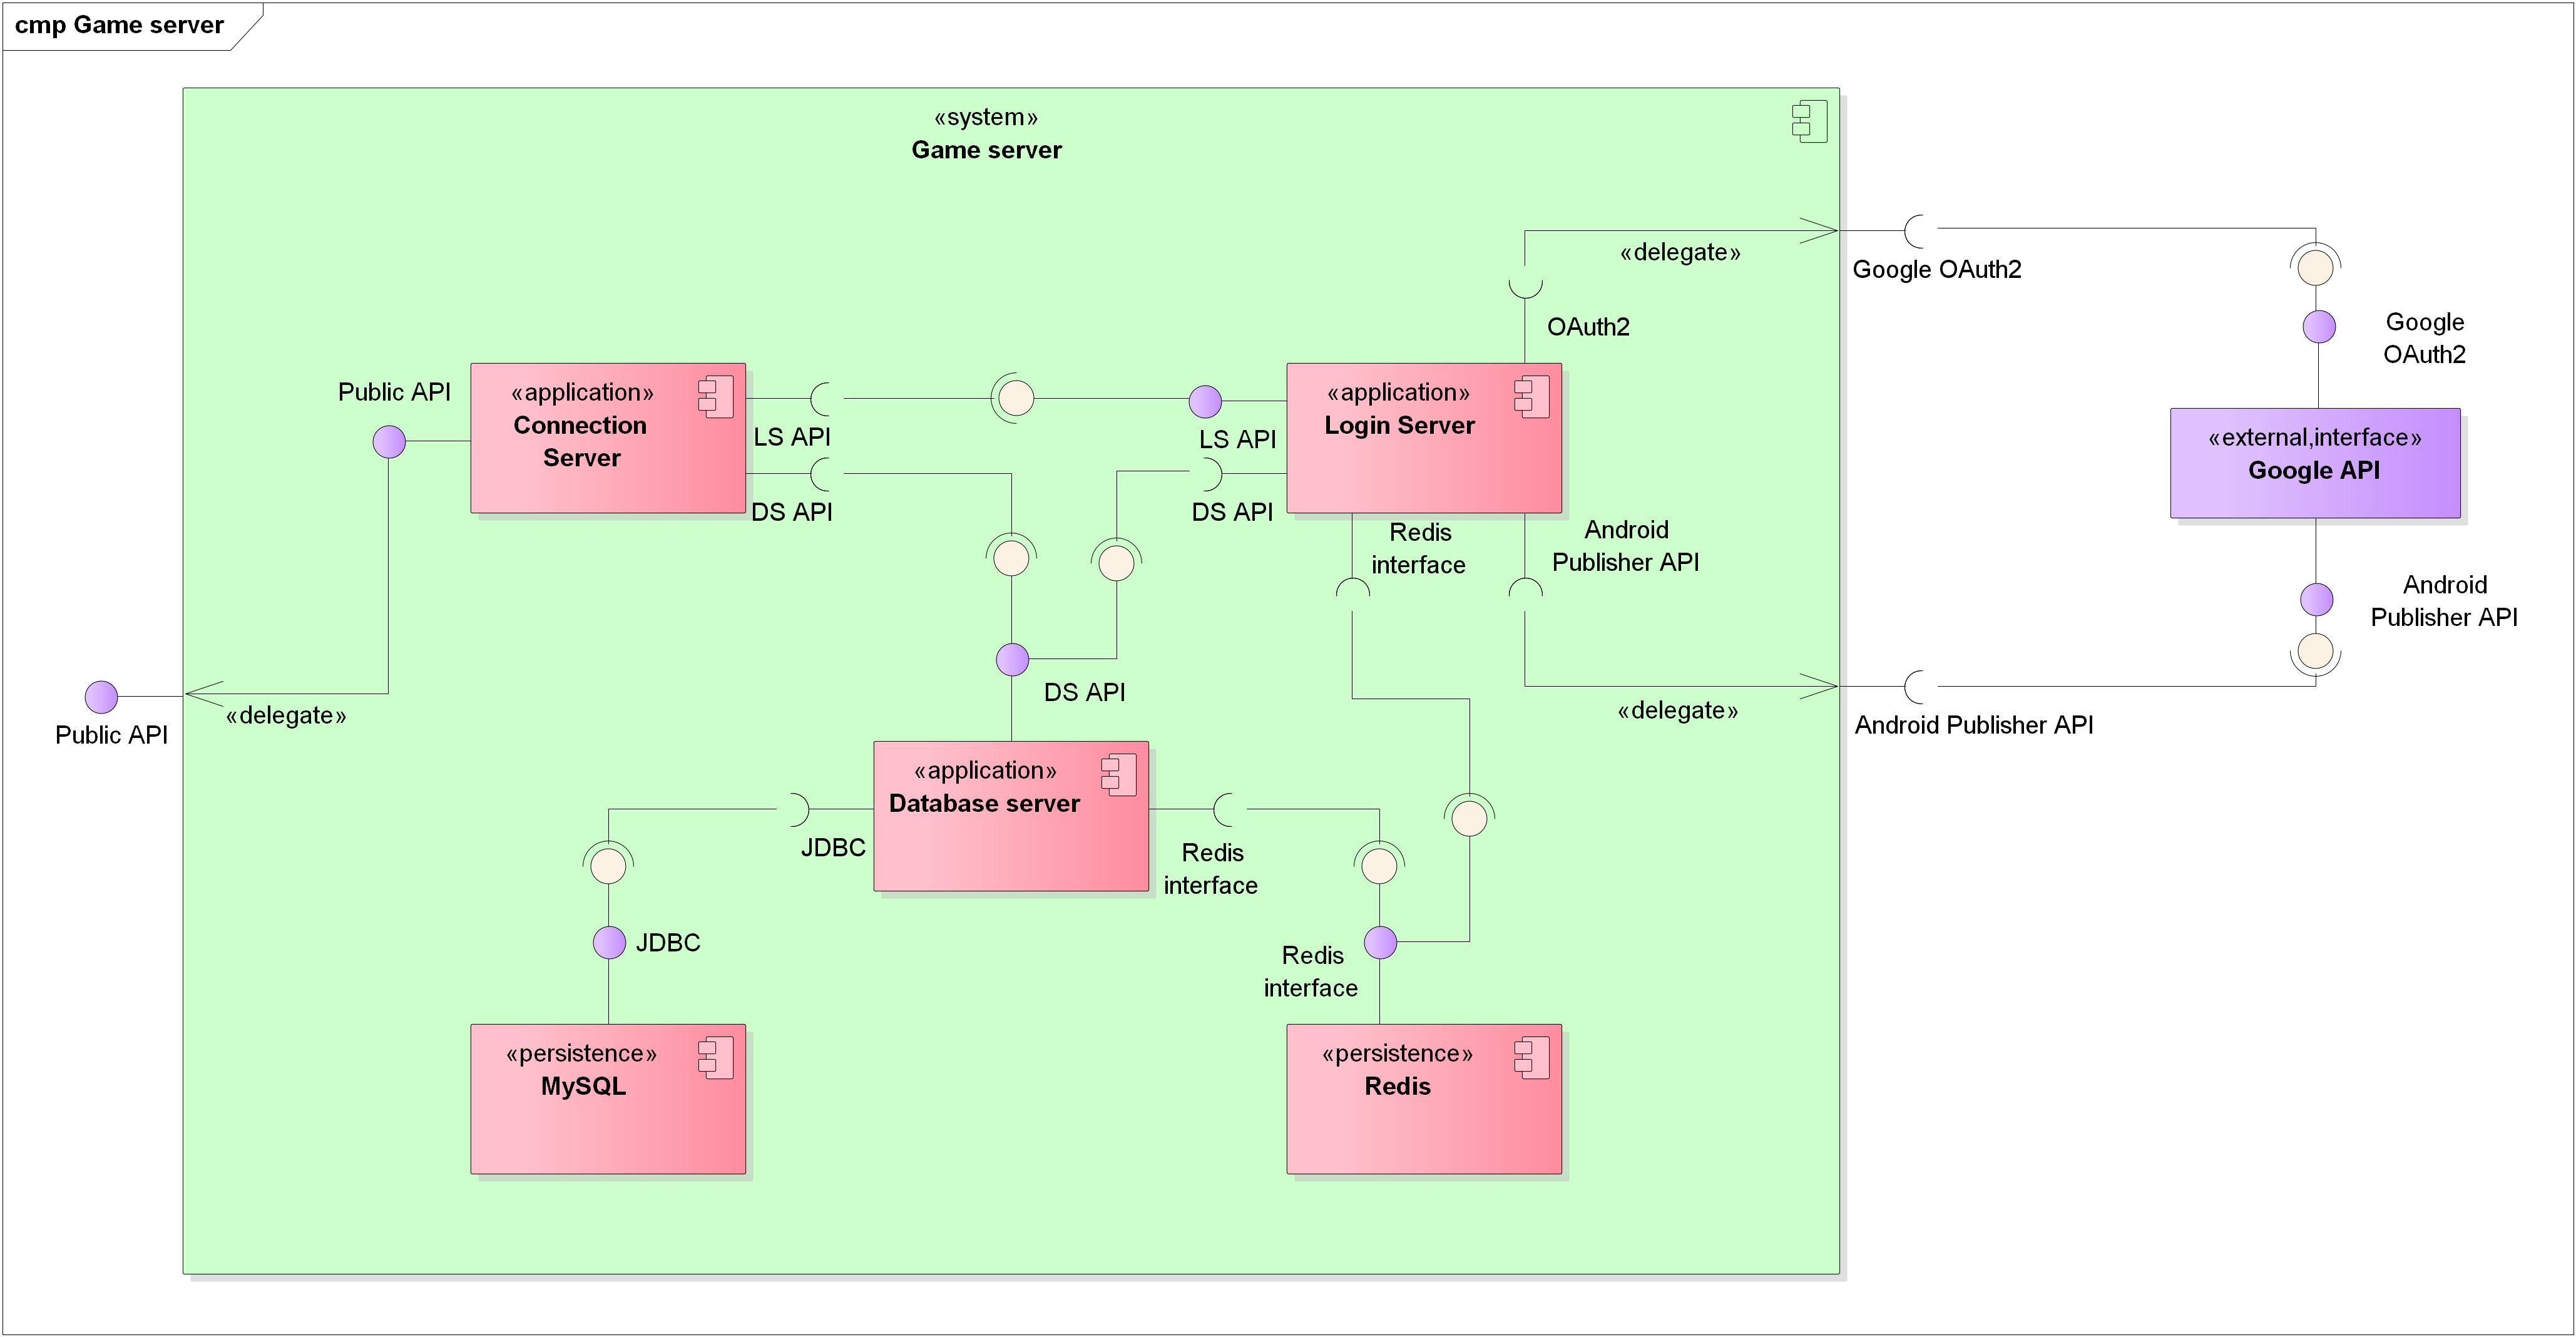
\includegraphics[width=\textwidth]{figures/Components}
	\centering			
	\caption{Component diagram of the~game server}
	\label{fig:components}
\end{figure}

	\subsection{Connection server}
	This is the~public entry point and the~only component exposed to clients. Reducing the~number of publicly accessible components increases security of the~server. CS handles all incoming traffic and delegates work to other components. 
	
	\subsection{Login server}
	The~main responsibility of the~LS is to handle user authentication and authorization. It connects to Redis where users' access codes are stored. The~LS is also used for in-app purchase verification. The~component is connected to Google API.
	
	\subsection{Database server}
	The~most important component is Database server. Most of the~game logic happens here. Since the~DS is responsible for data~persistence, it is connected to MySQL and Redis.

\section{Activities}
	\subsection{Authentication}
	Authentication process is visualized in Figure \ref{fig:adauth}.
	
	\begin{figure}[h]	
		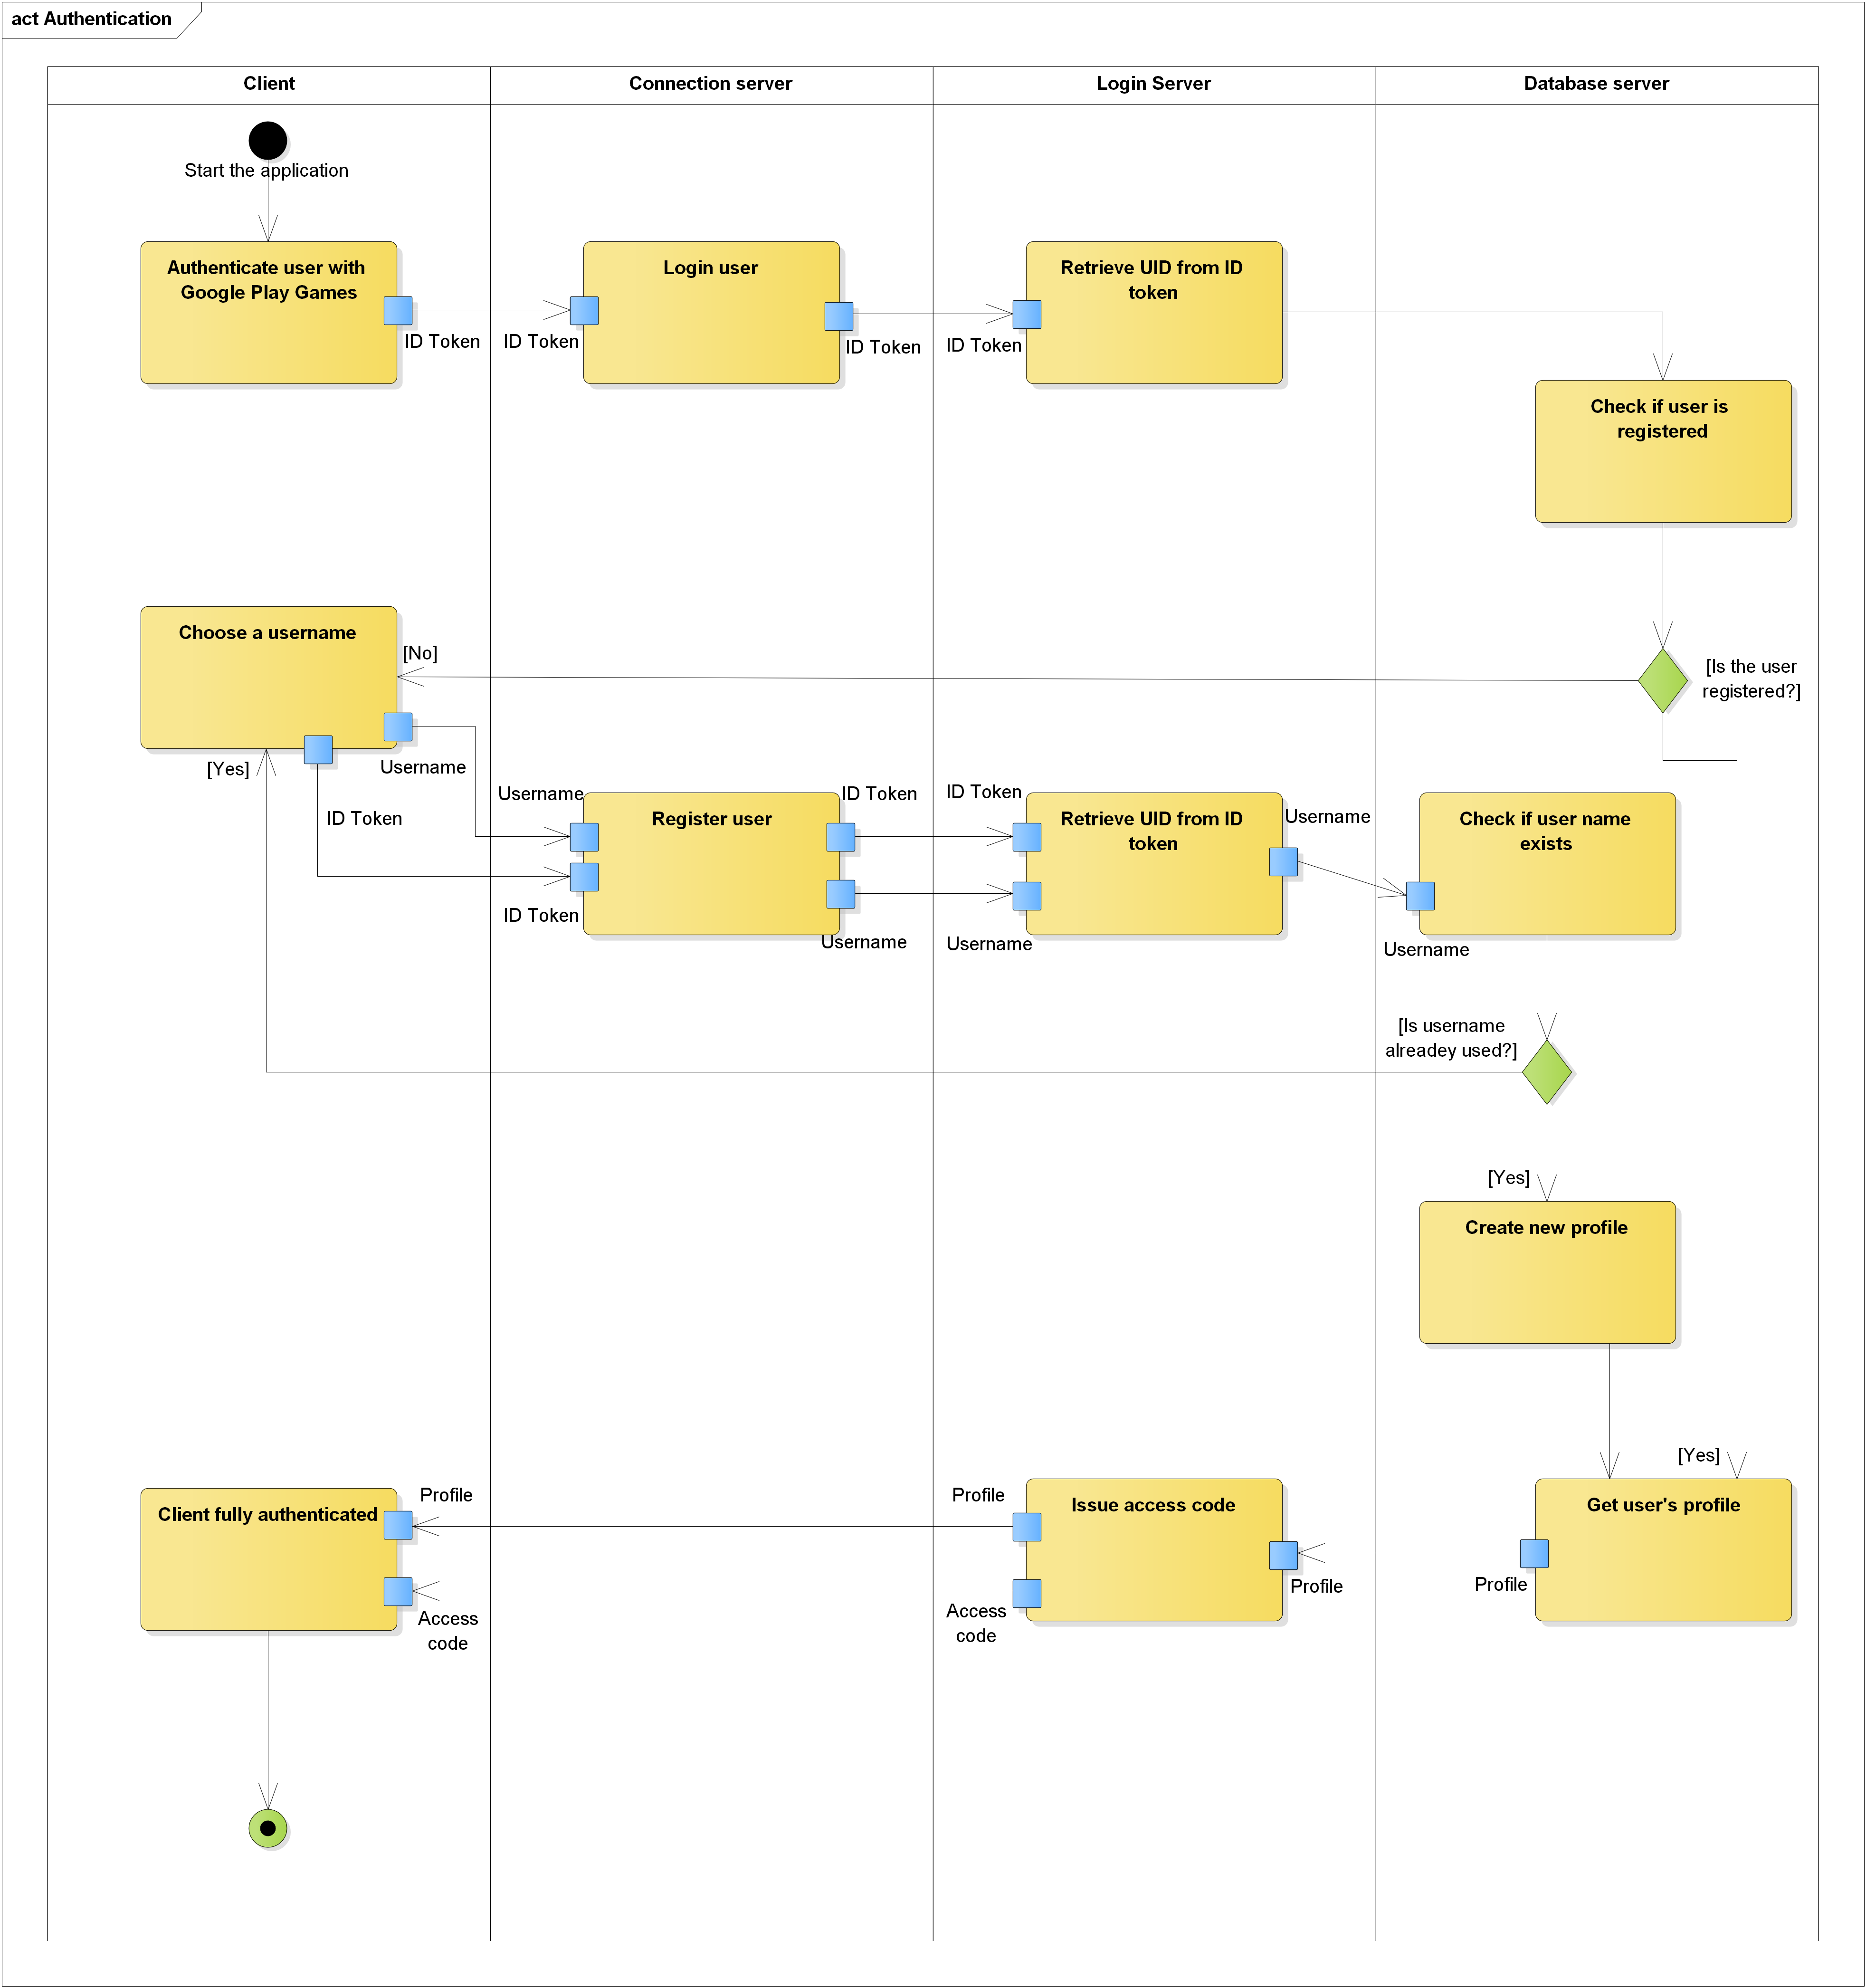
\includegraphics[width=\textwidth]{figures/AD_Authentication}
		\centering			
		\caption{Activity diagram of the~authentication process}
		\label{fig:adauth}
	\end{figure}

		\subsubsection{Access code}
		A~client is identified by his access code during a~session. The~code is random and unique. It is generated each time the~client finishes login process; the~old code,  previously issued to the~user, is invalidated.
		
		\subsubsection{Registration}
		Every user must register an account to gain access to the~game. The~user is asked to choose a~unique username. If the~username is already taken, the~whole registration process has to be repeated. LS retrieves user's UID and his e-mail address and passes the~information to the~DS, which then creates and initializes a~new user profile. Client is issued an access code and the~authentication process is completed.
		
		\subsubsection{Login}
		A~registered user can simply login using only his ID Token, which is provided to client during login process by Google Play Games. LS exchanges the~token for UID which is then used to retrieve user's profile. Client is issued an access code and the~authentication process is completed.
	
	\subsection{Killing a~monster}
	A user decides to fight a \textit{monster}. In this prototype, the client iteratively deals damage to the user and the \textit{monster}. The damage is calculated as \textit{attackDamage} attribute multiplied by a random value 0.5-1.5. If \textit{health} of the \textit{monster} drops to below zero before the user's one does, the \textit{monster} is killed. Server is notified of the result and rewards the user with \textit{gold} and \textit{experience}. The kill is logged, the \textit{monster} is removed from the game map and the client is provided with a one-time \textit{killConfirmationCode} which allows him to collect loot from the \textit{monster}.
		
	\subsection{Killing a~user}
	If user's \textit{health} drops to or below before the \textit{monster}'s one, the user dies. Client notifies the server of user's death. His \textit{health} is fully restored and he's punished with \textit{deathPenalty} which is deducted from his gold:  \[ deathPenalty = 200 + 100 * (userLevel - 1) \]
	
	\subsection{Collecting loot after kill}
	User is presented with an option to collect loot from a \textit{monster} he killed. Clients sends a \textit{killConfirmationCode} along with a list of items, he wants to collect, to the server. DS consumes the \textit{killConfirmationCode} and adds the selected items to user's inventory. Client then receives the updated inventory.
	
	\subsection{Buying an item}
	Client shows its user a \textit{shop} and lets him choose what item he wants to buy. The selected item is sent to the server. DS verifies the item is in the specified \textit{shop}. Price of the item is then deducted from user's account and the item is added to his inventory. If the user does not have enough \textit{gold}, the purchase is rejected and an error message is returned. Otherwise, client receives updated user's inventory.
	
	\subsection{Equipping an item}
	User selects a \textit{slot} and an appropriate item from his inventory. The client sends the item along with the slot to the server. DS checks if the item-slot pair is correct and assigns the item to the \textit{slot}. The successful result is then confirmed to the client.
	
	\subsection{Using an item}
	User selects a usable item from his inventory. Client sends the selected item to the server. DS decides what the item does by looking at attributes \textit{addHealth}, \textit{addExperience}, and \textit{addGold}. Based o the values set for the item, health, experience, and/or gold is added to user's account. The updated profile is then sent back to the client.
		
	\subsection{Purchasing in-app product}
	In-app purchases are handled on client which performs the transaction using a Google service. The prototype currently supports only buying \textit{gold}. If the transaction is successful, client sends a Google's \textit{Purchase token} to the server. LS verifies the status of the purchase using \textbf{Android Publisher API} \cite{androidpublisher} and adds the \textit{gold} to user's account. The purchase is then confirmed to the client.

	\subsection{Retrieving nearby game objects}
	Client visualizes nearby \textit{game objects} on the map. Since the user moves, the client frequently retrieves new \textit{game objects} based on the actual location, making high demands on the speed of the retrieval process.
	
	\begin{figure}[h]	
		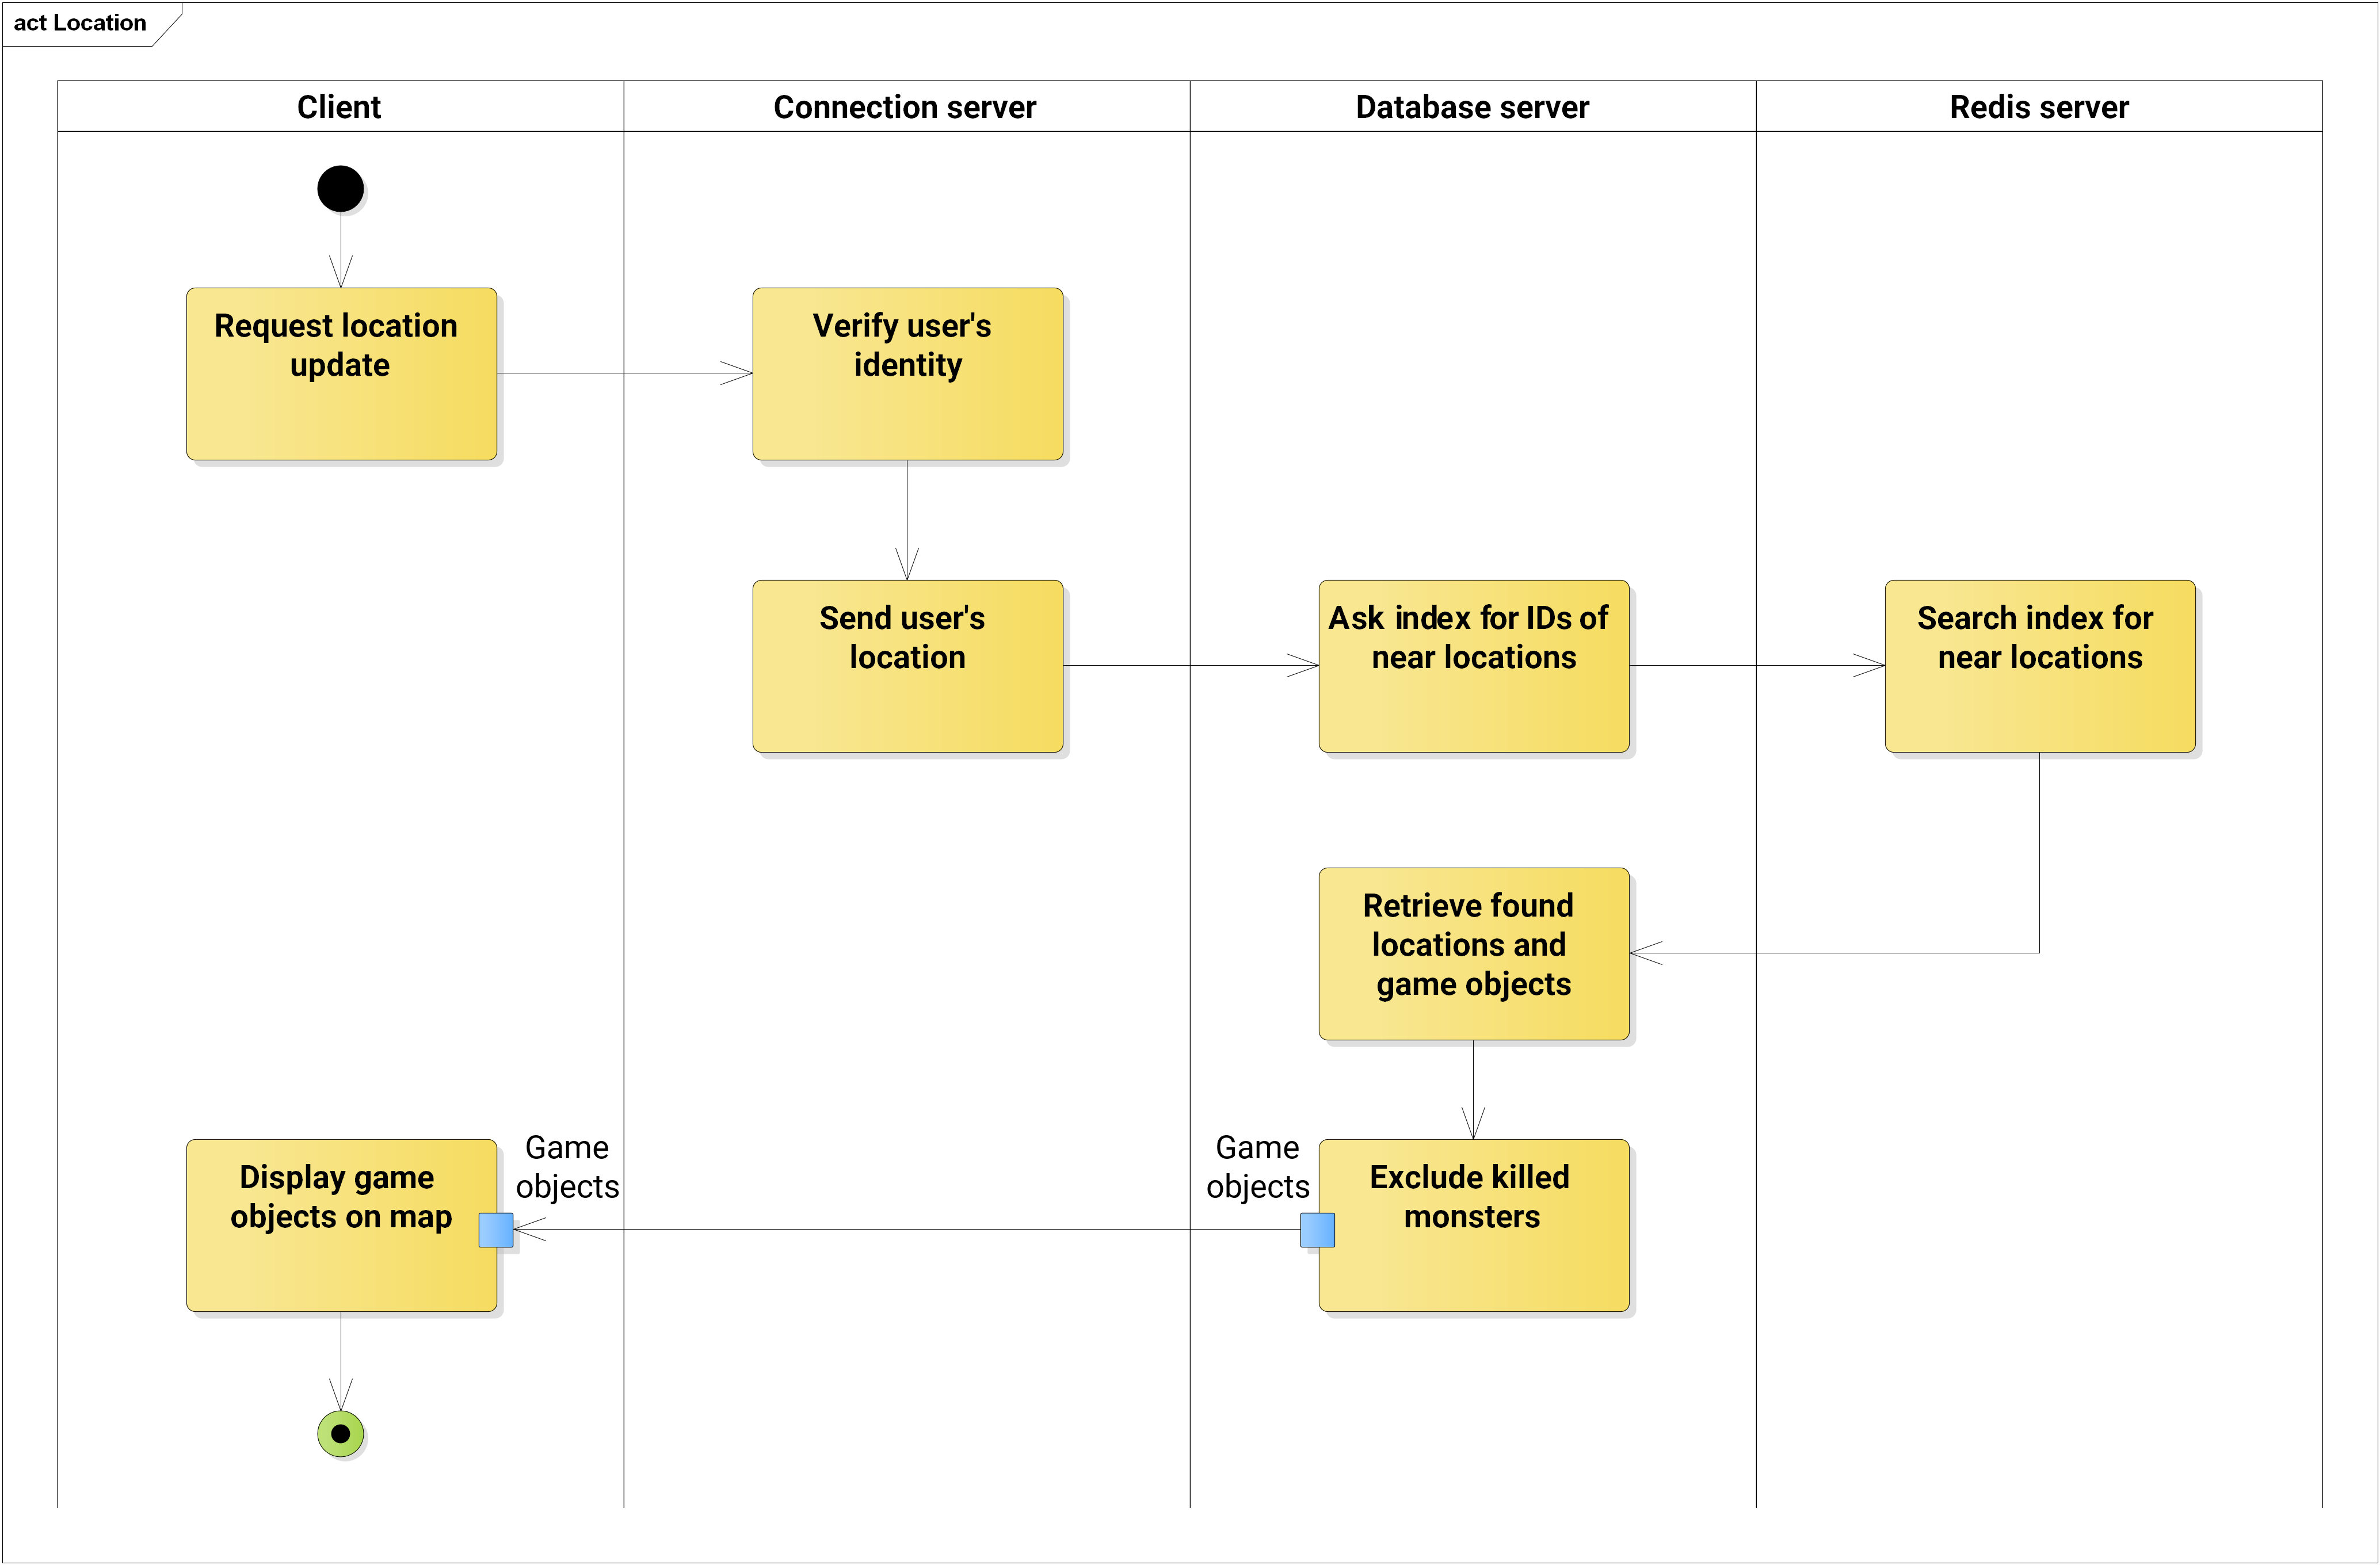
\includegraphics[width=\textwidth]{figures/AD_Location}
		\centering			
		\caption{Activity diagram of how the~server provides nearby game objects}
		\label{fig:adlocation}
	\end{figure} 
	
	Client sends its coordinates to the server. DS queries Redis which contains an index of all available \textit{locations}. The index responds with IDs of \textit{locations} in 200 m radius from the provided coordinates. The \textit{locations} and their assigned \textit{game objects} are then retrieved from the database. Server excludes already killed \textit{monsters}. The list of \textit{locations} and their \textit{game objects} is sent to the client which presents them on the map. See an activity diagram of the described process in Figure~\ref{fig:adlocation}.		

\section{Database Model}
	The database was designed to comply with the requirements specified in section \ref{section:requirements}. The entire database model is shown in Figure \ref{fig:dbmodel}. In the following text, I will describe important tables.	
	
	\begin{figure}[h]	
		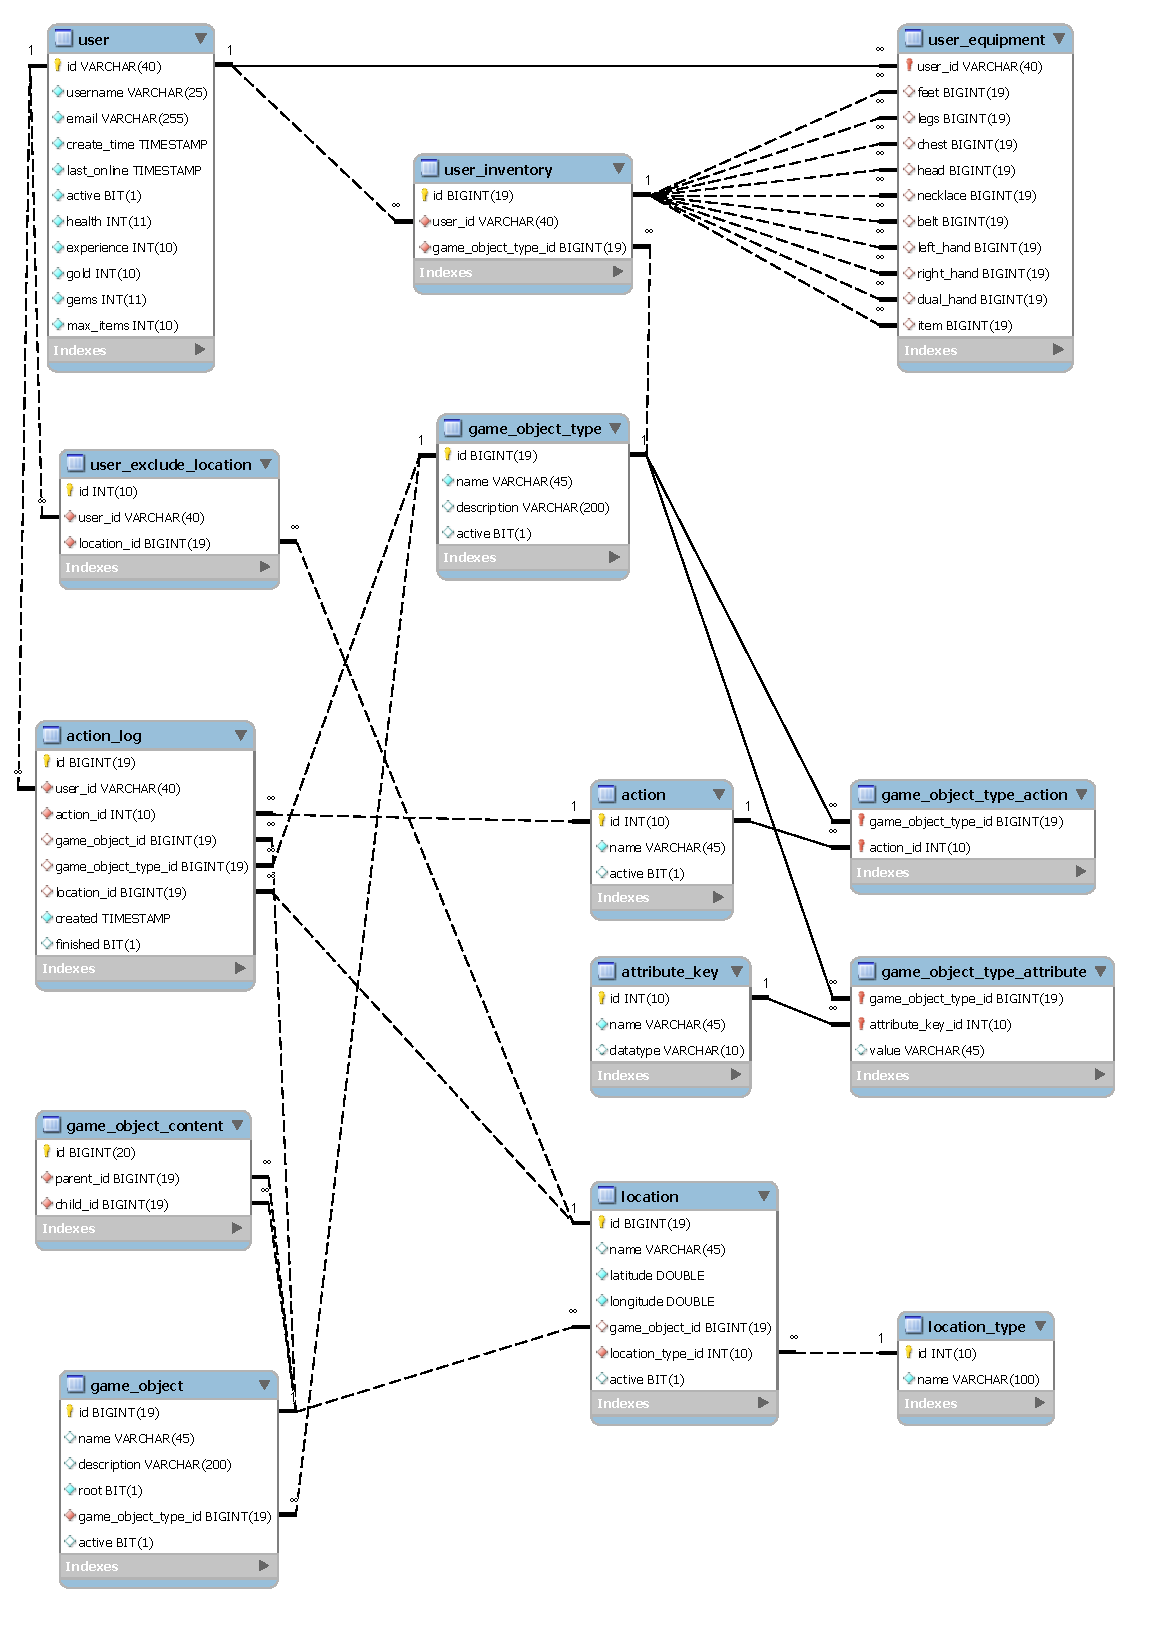
\includegraphics[width=\textwidth]{figures/DatabaseModel}
		\centering
		\caption{Database model}
		\label{fig:dbmodel}	
	\end{figure}
	
	\begin{description}
		\item[user] User's profile. It contains \textit{e-mail}, \textit{UID}, and \textit{username}. Quality attributes of the profile are also stored here - current \textit{health}, \textit{experience}, and \textit{gold}.
		
		\item[user\_inventory] Items a user own. 
		
		\item[user\_equipment] Information about what items a user has equipped. Is in 1:1 relationship with \textit{user}. Each column represents an equipment \textit{slot}. When an item is equipped, the item's entry from \textit{user\_inventory} to its \textit{slot}.
		
		\item[game\_object\_type] A "recipe" for every object in the game. Name and description of an object is stored here. The \textit{game\_object\_type} has linked attributes and actions.
	
		\item[action] Defines all allowed \textit{actions}. Each \textit{game object type} implements their subset.
		
		\item[game\_object\_type\_attribute] Defines all \textit{attributes} of a \textit{game object}. The attribute is identified by its \textit{name} and can have a \textit{value}.
	
		\item[game\_object] An implementation of \textit{game object type} which can be assigned to a \textit{location}.
	
		\item[game\_object\_content] Inventory of a \textit{game object}
	
		\item[location] Predefined real-world locations. Each one must have \textit{latitude} and \textit{longitude} defined; \textit{location} can have a \textit{game object} assigned. 
	
		\item[action\_log] Log of user's actions. In prototype, it is used only for kills to allow collecting loot.

		\item[user\_exclude\_location] Locations at which a user killed a monster. The table is periodically flushed. 
		
	\end{description}

\section{Administration}
The \textit{Database server} supports several API endpoints through which authorized administrators can manage the game data. The \textit{Admin} section is protected using \textbf{HTTP Basic Authentication} and thus the administrator has to know a valid username-password combination. For prototyping purposes, I've decided to provide only basic functionality for the administration.

	\subsection{Game object type management}
	Administrator can create new \textit{game object types} by sending a POST request to the endpoint \mbox{\textit{/admin/gameObjectType}}. A unique \textit{name} has to be specified for the new type. Optionally, the type can include a \textit{description}, a set of allowed \textit{actions} and \textit{attributes}.
	
	Existing \textit{game object types} can be updated. It is possible to change all their properties like \textit{name} and \textit{description}. Administrator can also add new \textit{attributes} and \textit{actions}. This is done using PUT request to the endpoint \mbox{\textit{/admin/gameObjectType}}
		
	All existing \textit{game object types} can be retrieved along with their \textit{actions} and \textit{attributes} by sending a GET request to the endpoint \mbox{\textit{/admin/gameObjectType}}
	
	\subsection{Game object management}
	Administrator can create new \textit{game objects} by sending a POST request to the endpoint \mbox{\textit{/admin/gameObject}}. \textit{Game object type} have to be specified for the new \textit{game object}. Optionally, the new object can have a set of children which can be later updated by calling PUT \mbox{\textit{/admin/gameObject}}.
	
	All existing \textit{game objects} can be retrieved along with their children by sending a GET request to the endpoint \mbox{\textit{/admin/gameObject}}
	
	\subsection{Location import}
	New locations can be imported from a file in OSM XML \cite{osmxml}. Administrator can do so be sending a POST request to \mbox{\textit{/admin/importLocations}}. The file is parsed for latitude and longitude data nad the new locations are inserted into the database.
	
	\subsection{Game object to a location assignment}
	A location serves no purpose without a\textit{game object} assigned to it. This can be achieved by using PUT endpoint \mbox{\textit{/admin/assignGameObjectToLocation}}.
	
	\subsection{Cache clearing}
	During the development process, developers might need to change game data by accessing the database directly. Since Hibernate won't be aware of such changes, its cache must be cleared via DELETE endpoint\mbox{\textit{/admin/clearCache}}.

\section{Calculations}
	\subsection{User's level}
	\[ level = \left\lfloor{\left(\frac{xp}{1024}\right)^{0.62} + 1}\right\rfloor, \]
	where $xp$ is user's experience.
	\subsection{Maximum health}
	Player's cannot exceed a certain value which linearly scales with his level.
	\[ maxHealth = 200 + 50 * (userLevel - 1) \]
	
	\subsection{Death penalty}
	A player is punished by losing gold when he dies. The total amount of the lost gold scales with user's level.
	\[ deathPenalty = 200 + 100 * (userLevel - 1) \]

\section{Public API}
Even though every component has its own API, only the~Connection Server API is available to clients. HTTP methods correspond to REST principles.

The~public API for the~prototype has been specified in cooperation with my colleague Tomáš Zahálka. Below are shortly described selected endpoints. For the~full list of publicly available API enpoints, please refer to Appendix~\ref{appendix:api}. The~mentioned appendix also contains description of API provided by LS and DS. 	

\subsection{GET /login}

The~Login endpoint verifies the~Google ID token and generates an~\textit{Access Code} for identification. When successfully authenticated, the~user's profile and the~\textit{Access Code} are returned.

\subsubsection*{Parameters}

\begin{description}

	\item[token] the~\textit{Google ID token}

\end{description}

\subsubsection*{Response}

\begin{description}

	\item[200] Successfully logged in, player's profile and the~\textit{Access Code} are returned.

	\item[403] Invalid token.

	\item[404] User not found, registration needed.

\end{description}

\subsection{POST /purchase}

The~Purchase endpoint offers support for in-app purchases. The~purchase is verified and then assigned to the~player. To be accepted, it cannot be cancelled or consumed.

\subsubsection*{Parameters}

\begin{description}

	\item[accessCode] the~\textit{Access Code}

	\item[productId] the~id of the~product to buy

	\item[token] the~purchase token

\end{description}

\subsubsection*{Response}

\begin{description}

	\item[200] Player's profile.

	\item[400] Invalid data.

	\item[403] Invalid \textit{Access Code} or the~purchase is not valid.

	\item[404] User not found, registration needed.

	\item[500] Unexpected error.

\end{description}

\subsection{GET /location}

This retrieves all nearby locations in a~200~m radius from the~provided coordinates. The~locations are returned along with their associated objects.

\subsubsection*{Parameters}

\begin{description}

	\item[lat] the~latitude

	\item[lon] the~longitude

	\item[accessCode] the~\textit{Access Code}

\end{description}

\subsubsection*{Response}

\begin{description}

	\item[200] List of nearby locations with game objects assigned to them.

	\item[500] Unexpected error.

\end{description}

\subsection{POST /action/kill}

The~kill action is performed on the~selected object and location. The~location is temporarily excluded from future requests to /location. The~player's health is updated, experience and gold are added. It returns a~\textit{killConfirmedCode} which is needed to perform the~collect action.

\subsubsection*{Parameters}

\begin{description}

	\item[accessCode] the~\textit{Access Code}

	\item[locationid] the~id of the~location

	\item[gameObjectId] the~id of the~game object

	\item[health] the~new player's health

\end{description}

\subsubsection*{Response}

\begin{description}

	\item[200] One-time code for kill confirmation.

	\item[400] Invalid data.

	\item[403] Invalid \textit{Access Code}.

	\item[404] User not found, registration needed.

	\item[500] Unexpected error.

\end{description}
	
	\chapter{Geo-data mining}
	Description of how the geographical data for the monsters and building will be obtained.

\section{Methodology}

\section{Output}
	
	\chapter{Implementation}
	\section{Development Environment}
I chose to use IntelliJ IDEA Ultimate 2017 \cite{idea} as my IDE. It is very user-friendly and powerful tool, which packs almost everything needed to develop a Java application. Build management is handled by Apache Maven \cite{maven}. This tool is extremely useful as it takes care of all application's dependencies and completely manages the build process. I also used GIT \cite{git} as my version control system. 

\section{Game Locations Source}
I have obtained all game locations from open-source project OpenStreetMaps (OSM) \cite{osm}. I downloaded complete map data of the Czech Republic. All features in OSM have one or more tags which specify a type of the feature, for example \textit{amenity.college} is a college or a campus building, \textit{historic.castle} is a castle and so on. Since it would be unreasonable to use all available features\footnote{The list of the feature types is available at \url{http://wiki.openstreetmap.org/wiki/Map_Features}}, I chose only several types, mostly from categories \textit{amenity} and \textit{historic}. I used a tool \textit{Osmosis} \cite{osmosis} to extract selected map features from the data. The selection resulted in 99~037 locations for the entire Czech Republic.

\section{Database}
The initial database structure was created from the database model in Figure \ref{fig:dbmodel}. I used MySQL Workbench \cite{mysqlworkbench} to generate a creation script.

The database includes an event which is triggered every 8 hours and wipes a table containing list of monsters killed by users. It causes the monsters to "re-spawn".  

\section{Project Structure}
The entire project is organized by its components (also called \textit{modules} in the IDEA's terminology). The project name is \textit{BachelorsServer} and consists of three modules -- \textit{ConnectionServer}, \textit{LoginServer}, and \textit{DatabaseServer}. Each module follows Maven's Standard Directory Layout\footnote{Described at \url{https://maven.apache.org/guides/introduction/introduction-to-the-standard-directory-layout.html}}. Top-level directory contains important configuration file. First one is \textit{config.yml} which stores server setting, such as listening ports, used protocol (HTTP/HTTPS), or URLs of other components. Path to this file must be specified as run argument of the server. Second file is \textit{pom.xml} (\textit{Project Object Model} file). It contains project-specific definitions for Maven. It specifies project version and name, its dependencies, and build strategies. 

Common package organization is\footnote{The package name \textit{module} is used as a placeholder for module-specific name.}:
\begin{description}
	\item[bachelors.\textit{module}] Main class and server configuration classes.
	\item[bachelors.\textit{module}.api] Classes used for JSON serialization and deserialization.
	\item[bachelors.\textit{module}.resources] Definitions of API endpoints.
\end{description}

\section{Connection Server}
A component which mostly serves as a proxy. It's implementation should be effective, since every client must connect to this component. Connection Server is the least complex module of the three. To satisfy the requirement for secured communication, this component allows incoming connection only using HTTPS.  

\subsection{Resources}
Classes which handle API requests. I described their main responsibilities and examples of their usage in the following text.

\begin{description}	
	\item[BaseResource] Abstract super-class for all resources. It contains commonly used methods, such as \textit{putRequest()}, or \textit{getRequest()}. These methods verify client's access code and delegates the request to a supplied URL.
	
	\item[UserResource] The class handles user-oriented requests. It is used to get user's profile, or his inventory.
	
	\item[LoginResource] The resource handles login and registration requests.
	
	\item[LocationResource] It is responsible for retrieving nearby game locations.
	
	\item[PurchaseResource] It is responsible for in-app purchases.

	\item[ActionResource] Important resource which processes user's action. It is used to kill a monster, to buy an item from a shop, or to use a health potion.
\end{description}

\section{Login Server}
A component responsible for authentication and authorization of clients and in-app purchase verification. I introduced several dependencies to help me fulfill the requirements.
 
\subsection{Access Key Store}
All client's requests after login are authorized using an \textit{access code}. The storage for these codes has to be fast, reliable and shared among all instances of Login Server component. The codes are stored in Redis and accessed from the component using a Redis java client -- Jedis \cite{jedis}. 

\subsection{Google API}
During the authentication process user sends a Google ID token. The component uses a Google API Client library \cite{googleapilibs} to access the API and exchange the token for user ID and e-mail. Similar process is the in-app purchase verification. The task is done using Google Play Developer API Client Library for Java  \cite{androidpublisherlibary}.

\section{Database Server}
The most complex and important component of the three. It is responsible for game logic and data persistence.

\subsection{Configuration Files}
A folder \textit{DatabaseServer/src/main/resources} contains configuration files for various dependencies of Database Server.
\begin{description}
	\item[hibernate.cfg.xml] Hibernate's configuraton. It defines second-level cache settings, type of the database engine, and lists database entities.
	\item[hibernate-redis.properties] Setup of Hibernate's second-level cache provider.
	\item[logback.xml] Setting of logger. Specifies what log level to show and where to output the logs.
	\item[redisson.yml] Configuration for Redisson which describes Redis server connection settings. 
\end{description}

\subsection{Hibernate}
The component uses Hibernate to access the database.

\subsubsection{Entities}
Every table in the database (except decomposed Many-to-Many relationships) has to be defined in an entity class. The specification contains not only table columns but also other entities in relationship with the class. It means the developer can for example simply call \textit{getGameObjectType()} on \textit{GameObjectEntity} and Hibernate automatically fetches associated \textit{GameObjectType} from the database.

\subsubsection{Second-level cache}
I've decided to use a second-level cache to optimize database interactions. Hibernate supports many cache providers and I chose to use hibernate-redis \cite{hibernateredis}. When the cache is configured, each entity can be annotated as \textit{@Cacheable} and have caching strategy specified. Hibernate then automatically caches the annotated entities.

\subsection{Models}
Package \textit{bachelors.database.db} contains model in which database operations are implemented. Each model extends abstract super-class \textit{BaseModel} and operates in its logical scope, e.g. \textit{UserModel} handles User-related operations, \textit{GamObjectObjectModel} handles GameObject-related operations and so on. The \textit{BaseModel} implements generic methods for simple database operations, like select all objects, or get object by id. Please refer to class diagram in Figure XXX or to project documentation for more detailed information about models.

\subsection{HTTP Basic Authentication} 
\textit{Admin} endpoints require a user to authenticate. Database Server use Dropwizard's authentication support. Only three additional files are needed to implement HTTP Basic Authentication. They are all located in package \textit{bachelors.database.security}. 
\begin{description}
	\item[AdminUser] Type of the user which extends \textit{java.security.Principal}.
	\item[AdminAuthenticator] The file defines how the application verifies user's username and password.
	\item[AdminAuthorizer] A method to verify if the user has sufficient privileges to access the requested resource.
\end{description}

\section{Deployment Environment}
\label{section:deploy}
The prototype currently runs on a virtual private server provided by WEDOS internet, a.s. The server runs on Debian~8. It uses the lowest available server specification\footnote{Offered server \url{https://hosting.wedos.com/cs/virtualni-servery.html}}:
\begin{tabbing}
	\textit{CPU} ~~ \= 1 thread Xeon 1.80 GHz\\
	\textit{RAM} \> 2 GB\\
	\textit{SSD} \> 15 GB\\
	\textit{SLA} \> 99.99\%
\end{tabbing}

The specifications are sufficient for testing and prototyping but in unused state, the server has only about 200~MB free RAM. Additionally, the application will have to support many concurrent users which requires more CPU threads.  
	
	\chapter{Deployment}
	\section{Deployment Diagram}
\begin{figure}[h]	
	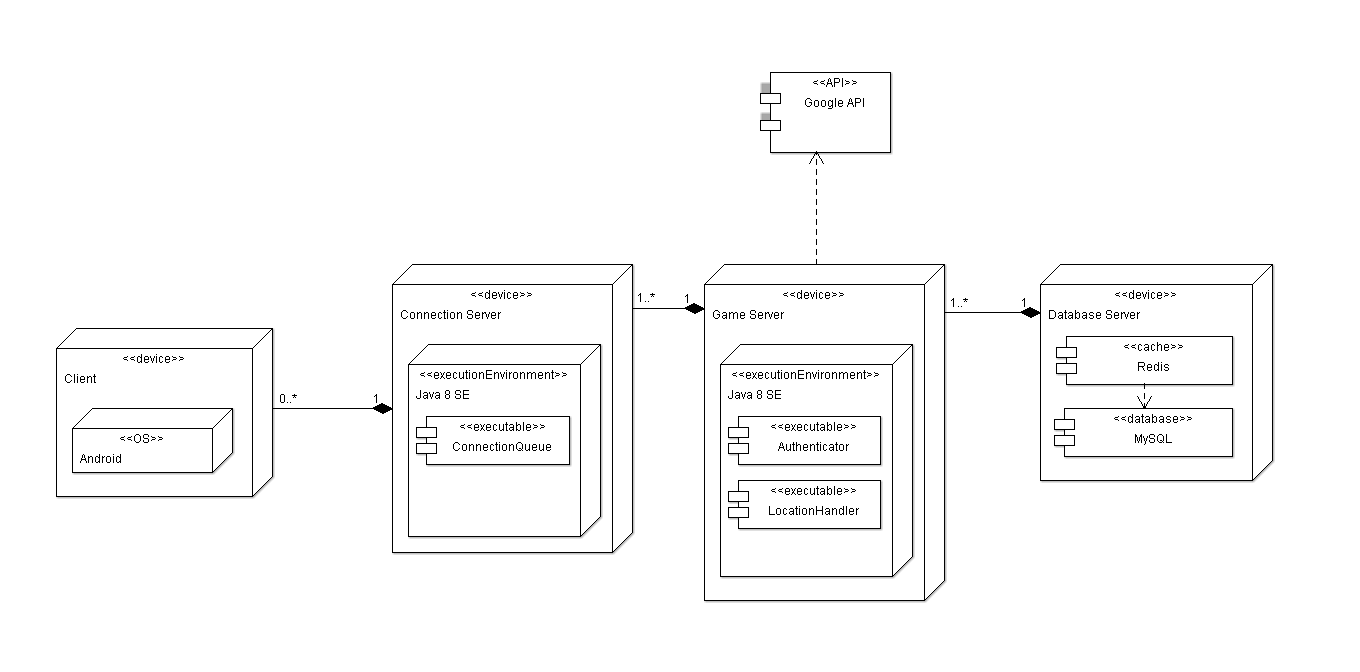
\includegraphics[width=\textwidth]{figures/DeploymentDiagram}
	\centering
	\caption{Deployment diagram for the game}
	
\end{figure}

	
	\chapter{Testing}
	\section{Unit Testing}
The project use JUnit \cite{junit}. Unit tests are located in \textit{src/test} directory in the root folder of each component and are included on the SD card. All components use the test to verify proper serialization and deserialization of JSON requests. Each tested JSON object is defined in \textit{src/test/resources/fixtures}.

The tests are packed in a test suite. This allows running all test by executing \textit{bachelors.*component\_name*.api.AllTests}. All tests are passing in the current build.

\section{Static Code Analysis}
I use SonarLint \cite{sonarlint} for on-the fly static code analysis. It offers many useful rules with specified severity and also a descriptions how to fix the issues. Static code analysis discovered many problems, the most notable were:
\begin{itemize}
	\item Create a private constructor to hide the implicit one in a static class.
	\item Use constant instead of duplicating string literal.
	\item Replace use of System.out by a logger.
	\item Make final constants also static.
\end{itemize}
The static analysis proved to be useful to maintain a good quality of the code and prevent bugs.

\section{System Testing}
I developed a Python script to test most of the endpoints in the real environment. The script doesn't test \textit{/login/registration} and \textit{/purchase} endpoints as they need valid Google tokens which can't be reused and are not easily obtainable. All tests are passing in the current build.

The script requires Python 3 or newer to run and is located in \textit{BachelorsServer/SystemTest/TestBachelorsPrototype.py}. The tester must initialize the script with values of a test account in the current database. The script then sends HTTP request to each endpoint testing valid and invalid data.

For example, test \textit{ACTION -- Kill} verifies the client cannot request setting his health to a negative value or more than his level allows. Script also tries to kill a monster at a wrong location and vice versa. A successful kill follows a second attempt to kill the same monster which must fail. 


\section{Client Testing}
I tested the application with my colleague using his client part of the game. We didn't discover any bugs which would affect the player in any way.

\section{Stress Testing}
I performed a stress test using Apache JMeter \cite{jmeter}. This testing framework is used to simulate interactions with a web server. Results of this type of test offer useful insight into how many concurrent users can server handle. Hardware specifications of the testing environment are described in Section \ref{section:deploy}.

I created a test plan in a way so that one thread simulates about 10 users. Each thread operates independently for 10 minutes and performs following series of actions:
\begin{enumerate}
	\item Wait 1 second\footnote{The locations are fetched from the server once every 10 seconds in the real game client},
	\item get nearby locations around location A (\textit{/location}),
	\item wait 1 second,
	\item get nearby locations around location B (\textit{/location}),
	\item wait 1 second,
	\item get nearby locations around location C (\textit{/location}),
	\item get profile (\textit{/user}),
	\item get inventory (\textit{/user/inventory}),
	\item go back to step 1.
\end{enumerate}

 As expected, calls to the endpoint \textit{/location} took the longest time out of the three tested, the difference in latency was about 30\% on average for up to 2~300 users. As you can see in Table \ref{tab:loadtestresults}, latency significantly increased at 3~000 users and about 2\% request resulted in an error. At 5 000 users, the server was far beyond its limits and responded with very high latency and about 8\% error rate. This behavior is expected due to the very limited resources of the server. The results might be affected by the performance issues of the test machine, since 500 threads had to be run concurrently to simulate 5 000 users.

Based on the test, server is currently able to handle more than 2~300 concurrent users with no performance issues that would affect clients. Since the server currently uses minimal available hardware specification, the computational power can be easily scaled up when the application reaches about 2~000 daily users.

\begin{table}
	\centering
	\begin{tabular}{r || c | c | c | c | c |}
		Users & 500 & 1 500 & 2 300 & 3 000 & 5 000 \\ \hline 
		Latency median [ms] & 108 & 123 & 166 & 473 & 1 737 \\
		Throughput [request/s] & 16.0 & 46.4 & 67.9 & 79.1 & 99.8 \\
	\end{tabular}
	\caption{Result of the server stress test.}
	\label{tab:loadtestresults}
\end{table}	


	
	
	\setsecnumdepth{part}
	\chapter{Results}
	
	
	\printbibliography

	
	\setsecnumdepth{all}
	\appendix
	
	\chapter{Acronyms}
	% \printglossaries
	\begin{description}
		\item[GUI] Graphical user interface
		\item[XML] Extensible markup language
	\end{description}
	
	
	\chapter{Contents of enclosed CD}
	
	%change appropriately
	
	\begin{figure}
		\dirtree{%
			.1 readme.txt\DTcomment{the file with CD contents description}.
			.1 exe\DTcomment{the directory with executables}.
			.1 src\DTcomment{the directory of source codes}.
			.2 wbdcm\DTcomment{implementation sources}.
			.2 thesis\DTcomment{the directory of \LaTeX{} source codes of the thesis}.
			.1 text\DTcomment{the thesis text directory}.
			.2 thesis.pdf\DTcomment{the thesis text in PDF format}.
			.2 thesis.ps\DTcomment{the thesis text in PS format}.
		}
	\end{figure}
	
\end{document}
